%
% This is an example LaTeX file which uses the SANDreport class file.
% It shows how a SAND report should be formatted, what sections and
% elements it should contain, and how to use the SANDreport class.
% It uses the LaTeX article class, but not the strict option.
% ItINLreport uses .eps logos and files to show how pdflatex can be used
%
% Get the latest version of the class file and more at
%    http://www.cs.sandia.gov/~rolf/SANDreport
%
% This file and the SANDreport.cls file are based on information
% contained in "Guide to Preparing {SAND} Reports", Sand98-0730, edited
% by Tamara K. Locke, and the newer "Guide to Preparing SAND Reports and
% Other Communication Products", SAND2002-2068P.
% Please send corrections and suggestions for improvements to
% Rolf Riesen, Org. 9223, MS 1110, rolf@cs.sandia.gov
%
\documentclass[pdf,12pt]{INLreport}
% pslatex is really old (1994).  It attempts to merge the times and mathptm packages.
% My opinion is that it produces a really bad looking math font.  So why are we using it?
% If you just want to change the text font, you should just \usepackage{times}.
% \usepackage{pslatex}
\usepackage{times}
\usepackage{longtable}
\usepackage[FIGBOTCAP,normal,bf,tight]{subfigure}
\usepackage{amsmath}
\usepackage{amssymb}
\usepackage[labelfont=bf]{caption}
\usepackage{pifont}
\usepackage{enumerate}
\usepackage{listings}
\usepackage{fullpage}
\usepackage{xcolor}          % Using xcolor for more robust color specification
\usepackage{ifthen}          % For simple checking in newcommand blocks
\usepackage{textcomp}
\usepackage{graphicx}
\usepackage{tabularx}
%\usepackage{authblk}         % For making the author list look prettier
%\renewcommand\Authsep{,~\,}

% Custom colors
\definecolor{deepblue}{rgb}{0,0,0.5}
\definecolor{deepred}{rgb}{0.6,0,0}
\definecolor{deepgreen}{rgb}{0,0.5,0}
\definecolor{forestgreen}{RGB}{34,139,34}
\definecolor{orangered}{RGB}{239,134,64}
\definecolor{darkblue}{rgb}{0.0,0.0,0.6}
\definecolor{gray}{rgb}{0.4,0.4,0.4}

\lstset {
  basicstyle=\ttfamily,
  frame=single
}

\setcounter{secnumdepth}{5}
\lstdefinestyle{XML} {
    language=XML,
    extendedchars=true,
    breaklines=true,
    breakatwhitespace=true,
%    emph={name,dim,interactive,overwrite},
    emphstyle=\color{red},
    basicstyle=\ttfamily,
%    columns=fullflexible,
    commentstyle=\color{gray}\upshape,
    morestring=[b]",
    morecomment=[s]{<?}{?>},
    morecomment=[s][\color{forestgreen}]{<!--}{-->},
    keywordstyle=\color{cyan},
    stringstyle=\ttfamily\color{black},
    tagstyle=\color{darkblue}\bf\ttfamily,
    morekeywords={name,type},
%    morekeywords={name,attribute,source,variables,version,type,release,x,z,y,xlabel,ylabel,how,text,param1,param2,color,label},
}
\lstset{language=python,upquote=true}

\usepackage{titlesec}
\newcommand{\sectionbreak}{\clearpage}
\setcounter{secnumdepth}{4}

%\titleformat{\paragraph}
%{\normalfont\normalsize\bfseries}{\theparagraph}{1em}{}
%\titlespacing*{\paragraph}
%{0pt}{3.25ex plus 1ex minus .2ex}{1.5ex plus .2ex}

%%%%%%%% Begin comands definition to input python code into document
\usepackage[utf8]{inputenc}

% Default fixed font does not support bold face
\DeclareFixedFont{\ttb}{T1}{txtt}{bx}{n}{9} % for bold
\DeclareFixedFont{\ttm}{T1}{txtt}{m}{n}{9}  % for normal

\usepackage{listings}

% Python style for highlighting
\newcommand\pythonstyle{\lstset{
language=Python,
basicstyle=\ttm,
otherkeywords={self, none, return},             % Add keywords here
keywordstyle=\ttb\color{deepblue},
emph={MyClass,__init__},          % Custom highlighting
emphstyle=\ttb\color{deepred},    % Custom highlighting style
stringstyle=\color{deepgreen},
frame=tb,                         % Any extra options here
showstringspaces=false            %
}}


% Python environment
\lstnewenvironment{python}[1][]
{
\pythonstyle
\lstset{#1}
}
{}

% Python for external files
\newcommand\pythonexternal[2][]{{
\pythonstyle
\lstinputlisting[#1]{#2}}}

\lstnewenvironment{xml}
{}
{}

% Python for inline
\newcommand\pythoninline[1]{{\pythonstyle\lstinline!#1!}}

% Named Colors for the comments below (Attempted to match git symbol colors)

\def\DRAFT{} % Uncomment this if you want to see the notes people have been adding
% Comment command for developers (Should only be used under active development)
\ifdefined\DRAFT
  \newcommand{\nameLabeler}[3]{\textcolor{#2}{[[#1: #3]]}}
\else
  \newcommand{\nameLabeler}[3]{}
\fi
% Commands for making the LaTeX a bit more uniform and cleaner
\newcommand{\TODO}[1]    {\textcolor{red}{\textit{(#1)}}}
\newcommand{\xmlAttrRequired}[1] {\textcolor{red}{\textbf{\texttt{#1}}}}
\newcommand{\xmlAttr}[1] {\textcolor{cyan}{\textbf{\texttt{#1}}}}
\newcommand{\xmlNodeRequired}[1] {\textcolor{deepblue}{\textbf{\texttt{<#1>}}}}
\newcommand{\xmlNode}[1] {\textcolor{darkblue}{\textbf{\texttt{<#1>}}}}
\newcommand{\xmlString}[1] {\textcolor{black}{\textbf{\texttt{'#1'}}}}
\newcommand{\xmlDesc}[1] {\textbf{\textit{#1}}} % Maybe a misnomer, but I am
                                                % using this to detail the data
                                                % type and necessity of an XML
                                                % node or attribute,
                                                % xmlDesc = XML description
\newcommand{\default}[1]{~\\*\textit{Default: #1}}
\newcommand{\nb} {\textcolor{deepgreen}{\textbf{~Note:}}~}

%%%%%%%% End comands definition to input python code into document

%\usepackage[dvips,light,first,bottomafter]{draftcopy}
%\draftcopyName{Sample, contains no OUO}{70}
%\draftcopyName{Draft}{300}

% The bm package provides \bm for bold math fonts.  Apparently
% \boldsymbol, which I used to always use, is now considered
% obsolete.  Also, \boldsymbol doesn't even seem to work with
% the fonts used in this particular document...
\usepackage{bm}

% Define tensors to be in bold math font.
\newcommand{\tensor}[1]{{\bm{#1}}}

% Override the formatting used by \vec.  Instead of a little arrow
% over the letter, this creates a bold character.
\renewcommand{\vec}{\bm}

% Define unit vector notation.  If you don't override the
% behavior of \vec, you probably want to use the second one.
\newcommand{\unit}[1]{\hat{\bm{#1}}}
% \newcommand{\unit}[1]{\hat{#1}}

% Use this to refer to a single component of a unit vector.
\newcommand{\scalarunit}[1]{\hat{#1}}

% \toprule, \midrule, \bottomrule for tables
\usepackage{booktabs}

% \llbracket, \rrbracket
\usepackage{stmaryrd}

\usepackage{hyperref}
\hypersetup{
    colorlinks,
    citecolor=black,
    filecolor=black,
    linkcolor=black,
    urlcolor=black
}

\newcommand{\wiki}{\href{https://github.com/idaholab/raven/wiki}{RAVEN wiki}}

% Compress lists of citations like [33,34,35,36,37] to [33-37]
\usepackage{cite}

% If you want to relax some of the SAND98-0730 requirements, use the "relax"
% option. It adds spaces and boldface in the table of contents, and does not
% force the page layout sizes.
% e.g. \documentclass[relax,12pt]{SANDreport}
%
% You can also use the "strict" option, which applies even more of the
% SAND98-0730 guidelines. It gets rid of section numbers which are often
% useful; e.g. \documentclass[strict]{SANDreport}

% The INLreport class uses \flushbottom formatting by default (since
% it's intended to be two-sided document).  \flushbottom causes
% additional space to be inserted both before and after paragraphs so
% that no matter how much text is actually available, it fills up the
% page from top to bottom.  My feeling is that \raggedbottom looks much
% better, primarily because most people will view the report
% electronically and not in a two-sided printed format where some argue
% \raggedbottom looks worse.  If we really want to have the original
% behavior, we can comment out this line...
\raggedbottom
\setcounter{secnumdepth}{5} % show 5 levels of subsection
\setcounter{tocdepth}{5} % include 5 levels of subsection in table of contents

% ---------------------------------------------------------------------------- %
%
% Set the title, author, and date
%
\title{HYBRID User Manual}
%\author{%
%\begin{tabular}{c} Author 1 \\ University1 \\ Mail1 \\ \\
%Author 3 \\ University3 \\ Mail3 \end{tabular} \and
%\begin{tabular}{c} Author 2 \\ University2 \\ Mail2 \\ \\
%Author 4 \\ University4 \\ Mail4\\
%\end{tabular} }


\author{
 \\Konor Frick\\
 \\Andrea Alfonsi\\
 \\Cristian Rabiti\\
 \\Daniel Mikkelson\\
}
% \\James B. Tompkins}   Just people who actually ``developed'' a significant capability in the code should be placed here. Andrea
%\author{\textbf{\textit{Main Developers:}}  \\Andrea Alfonsi}
%\author{\\Joshua Cogliati}
%\author{\\Diego Mandelli}
%\author{\\Robert Kinoshita}
%\author{\\Sonat Sen}
%
%\author{Cristian Rabiti}
%\author{Andrea Alfonsi}
%\author{Joshua Cogliati}
%\author{Diego Mandelli}
%\author{Robert Kinoshita}
%\author{Sonat Sen}
%\affil{Idaho National Laboratory, Idaho Falls, ID 83402}
%\\\{cristian.rabiti, andrea.alfonsi, joshua.cogliati, diego.mandelli, robert.kinoshita, ramazan.sen\}@inl.gov}

% There is a "Printed" date on the title page of a SAND report, so
% the generic \date should [WorkingDir:]generally be empty.
\date{}


% ---------------------------------------------------------------------------- %
% Set some things we need for SAND reports. These are mandatory
%
\SANDnum{INL/MIS-20-60624}
\SANDprintDate{\today}
\SANDauthor{Konor Frick, Andrea Alfonsi, Cristian Rabiti, Daniel Mikkelson}
\SANDreleaseType{Revision 1}

% ---------------------------------------------------------------------------- %
% Include the markings required for your SAND report. The default is "Unlimited
% Release". You may have to edit the file included here, or create your own
% (see the examples provided).
%
% \include{MarkOUO} % Not needed for unlimted release reports

\def\component#1{\texttt{#1}}

% ---------------------------------------------------------------------------- %
\newcommand{\systemtau}{\tensor{\tau}_{\!\text{SUPG}}}

% Added by Sonat
\usepackage{placeins}
\usepackage{array}

\newcolumntype{L}[1]{>{\raggedright\let\newline\\\arraybackslash\hspace{0pt}}m{#1}}
\newcolumntype{C}[1]{>{\centering\let\newline\\\arraybackslash\hspace{0pt}}m{#1}}
\newcolumntype{R}[1]{>{\raggedleft\let\newline\\\arraybackslash\hspace{0pt}}m{#1}}

% end added by Sonat
% ---------------------------------------------------------------------------- %
%
% Start the document
%

\begin{document}
\pagenumbering{roman} % switch to roman numerals
    \maketitle

    % ------------------------------------------------------------------------ %
    % An Abstract is required for SAND reports
    %
%    \begin{abstract}
%    \input abstract
%    \end{abstract}


    % ------------------------------------------------------------------------ %
    % An Acknowledgement section is optional but important, if someone made
    % contributions or helped beyond the normal part of a work assignment.
    % Use \section* since we don't want it in the table of context
    %
%    \clearpage
%    \section*{Acknowledgment}



%	The format of this report is based on information found
%	in~\cite{Sand98-0730}.


    % ------------------------------------------------------------------------ %
    % The table of contents and list of figures and tables
    % Comment out \listoffigures and \listoftables if there are no
    % figures or tables. Make sure this starts on an odd numbered page
    %
    \cleardoublepage		% TOC needs to start on an odd page
    \tableofcontents
    %\listoffigures
    %\listoftables


    % ---------------------------------------------------------------------- %
    % An optional preface or Foreword
%    \clearpage
%    \section*{Preface}
%    \addcontentsline{toc}{section}{Preface}
%	Although muggles usually have only limited experience with
%	magic, and many even dispute its existence, it is worthwhile
%	to be open minded and explore the possibilities.


    % ---------------------------------------------------------------------- %
    % An optional executive summary
    %\clearpage
    %\section*{Summary}
    %\addcontentsline{toc}{section}{Summary}
    %\input{Summary.tex}
%	Once a certain level of mistrust and skepticism has
%	been overcome, magic finds many uses in todays science



%	and engineering. In this report we explain some of the
%	fundamental spells and instruments of magic and wizardry. We
%	then conclude with a few examples on how they can be used
%	in daily activities at national Laboratories.


    % ---------------------------------------------------------------------- %
    % An optional glossary. We don't want it to be numbered
%    \clearpage
%    \section*{Nomenclature}
%    \addcontentsline{toc}{section}{Nomenclature}
%    \begin{description}
%          \item[alohomoral]
%           spell to open locked doors and containers
%          \item[leviosa]
%           spell to levitate objects
%    \item[remembrall]
%           device to alert you that you have forgotten something
%    \item[wand]
%           device to execute spells
%    \end{description}


    % ---------------------------------------------------------------------- %
    % This is where the body of the report begins; usually with an Introduction
    %
    \SANDmain		% Start the main part of the report
\pagenumbering{arabic} % switch to arabic numerals, start over at "1"
\section{Introduction}
% High-level HYBRID description
One of the goals of the HYBRID modeling and simulation project is to assess the economic viability of hybrid systems in a market that contains renewable energy sources like wind. The hybrid system would be a nuclear reactor that not only generates electricity, but also provides heat to another plant that produces by-products, like hydrogen or desalinated water. The idea is that the possibility of selling heat to a heat user absorbs (at least part of) the market volatility introduced by the renewable energy sources.

The system that is studied is modular and made of an assembly of components. For example, a system could contain a hybrid nuclear reactor, a gas turbine, a battery and some renewables. This system would correspond to the size of a balance area, but in theory any size of system is imaginable. The system is modeled in the ‘Modelica/Dymola’ language.
To assess the economics of the system, an optimization procedure is varying different parameters of the system and tries to find the minimal cost of electricity production.

\subsection{Modelica Models}
Idaho National Laboratory (INL) has been developing the NHES package, a library of high-fidelity process models in the commercial Modelica language platform Dymola since early 2013 \cite{2017Report}, \cite{2016HTSE}, \cite{2018ThermalStorage}, \cite{2019NuScaleM4}. The Modelica language is a non-proprietary, object oriented, equation-based language that is used to conveniently model complex, physical systems. Modelica is an inherently time-dependent modeling language that allows the swift interconnection of independently developed models. Being an equation-based modeling language that employs differential algebraic equation (DAE) solvers, users can focus on the physics of the problem rather than the solving technique used, allowing faster model generation and ultimately analysis. This feature alongside system flexibility has led to the widespread use of the Modelica language across industry for commercial applications. System interconnectivity and the ability to quickly develop novel control strategies while still encompassing overall system physics is why INL has chosen to develop the Integrated Energy Systems (IES) framework in the Modelica language.

\subsection{Individual Components}
The current version of the NHES library employs both third party components from the Modelica Standard Library \cite{ModelicaAssociation} and TRANSFORM \cite{TRANSFORM} and components developed internal to the project for specific subsystems. For example, the NHES library contains a large variety of models for the development of a high-temperature steam electrolysis plant, a gas turbine, a basic Rankine cycle balance of plant, and a light water nuclear reactor. Components included in the library that support the development of these systems include 1-D pipes, pressurizers, condensers, turbines (steam and gas), heat exchangers, a simple logic-based battery, a nuclear fuel subchannel, etc. Third party models include numerous additional models including source/sink components (e.g., fluid boundary conditions), additional heat exchanger models, logical components for control system development, multi-body components, additional supporting functions (e.g., LAPACK, interpolation, smoothing), etc. Please see the specific libraries for additional information. 

\subsection{Hybrid Requirements}


The repository itself can be found here: \url{https://hpcgitlab.inl.gov/hybrid/hybrid}
 
\textbf{Software requirements are as follows:}

\begin{enumerate}
\item Commercial Modelica platform Dymola -- \url{https://www.3ds.com/products-services/catia/products/dymola/latest-release/}.
\item Risk Analysis and Virtual ENviroment (RAVEN) -- \url{https://raven.inl.gov/SitePages/Software%20Infrastructure.aspx}
\item Python 3 -- \url{https://docs.conda.io/en/latest/miniconda.html}
\item Microsoft Visual Studio Community Edition. -- \url{https://visualstudio.microsoft.com/downloads/}
\end{enumerate}

	

\textbf{Note}: Steps 3 and 4 can be accomplished by following the RAVEN installation instructions in step two. The installation procedure will be outlined below. 
All physical models are run within the Dymola simulation framework graphical user interface (GUI).  Background information on the Modelica as a language as well as good general guidance on coding practices can be found at the two references shown below. 
\begin{enumerate}
\item \url{https://webref.modelica.university/}
\item \url{https://mbe.modelica.university/}
\end{enumerate}


%\section{Manual Formats}
In order to highlight some parts of the Manual having a particular meaning (e.g. input structure, examples, terminal commands, etc.), specific formats have been used. In this sections all the formats with a specific meaning are reported:
\begin{itemize}
\item \textbf{\textit{Python Coding:}}
\begin{lstlisting}[language=python]
class AClass():
  def aMethodImplementation(self):
    pass
\end{lstlisting}
\item \textbf{\textit{XML input example:}}
\begin{lstlisting}[style=XML,morekeywords={anAttribute}]
<MainXMLBlock>
  ...
  <anXMLnode name='anObjectName' anAttribute='aValue'>
     <aSubNode>body</aSubNode>
  </anXMLnode>
  ...
</MainXMLBlock>
\end{lstlisting}
\item \textbf{\textit{Bash Commands:}}
\begin{lstlisting}[language=bash]
cd trunk/raven/
./raven_libs_script.sh
cd ../../
\end{lstlisting}
\end{itemize}


% definitions

% content
\section{HYBRID Installation Procedure}
\subsection{Overview}

The installation of the HYBRID repository is a straightforward procedure;
depending on the usage purpose and machine architecture, the
installation process slightly differs.

In the following sections, the recommended installation procedure is outlined.  For alternatives, we encourage
checking the \wiki.  The windows 10 machine on which
HYBRID is tested and developed, uses the standard installation procedures outlined below.

The installation process will involve four steps:
\begin{itemize}
  \item Installing prerequisites, which depends on your operating system;
  \item Installing conda;
  \item Installing RAVEN.
  \item Installing HYBRID.
\end{itemize}

\subsection{Cloning the Hybrid Repository}
\label{sec:clone raven}

The first step in installing the package is to clone the HYBRID repository. To do this, use
\begin{lstlisting}[language=bash]
git clone https://github.com/idaholab/HYBRID.git
\end{lstlisting}
This will download the repository into a folder called 'hybrid'. To go inside the folder, use
\begin{lstlisting}[language=bash]
cd hybrid
\end{lstlisting}


\subsubsection{Install RAVEN and its plugins as a sub-module}

The next step is to download and install RAVEN and the submodule (e.g. TEAL, HERON) plugins as a sub-module of the HYBRID repository. 

A submodule allows you to keep another Git repository in a subdirectory of your repository. The other repository has its own history, which does not interfere with the history of the current repository. This can be used to have external dependencies such as third party libraries for example.

In order to get RAVEN do the following in the hybrid folder

\begin{lstlisting}[language=bash]
git checkout devel
\end{lstlisting}

Update the Branch

\begin{lstlisting}[language=bash]
git pull
\end{lstlisting}

to add RAVEN as a submodule
\begin{lstlisting}[language=bash]
git submodule update --init --recursive
\end{lstlisting}

\textbf{Install and Compile RAVEN. }
Once you have downloaded RAVEN as a sub-module, you have to install it. go to the \href{https://github.com/idaholab/raven/wiki/intallationMain}{RAVEN Wiki} for information about how to install it. Run all the tests outlined in the RAVEN wiki. 

\subsubsection{Inform the Framework Paths}

In order to set up the hybrid repository, you must inform the framework about the location of the Dymola python interface. For doing so, navigate to the hybrid directory:

to add RAVEN as a submodule
\begin{lstlisting}[language=bash]
cd <path to your hybrid repository>/hybrid
\end{lstlisting}
Run the following command:
\begin{lstlisting}[language=bash]
./scripts/write_hybridrc.py -p DYMOLA_PATH
\end{lstlisting}

Where DYMOLAPATH is the path to the python interface egg folder in the DYMOLA installation locally. For example:
 
\begin{lstlisting}[language=bash]
./scripts/write_hybridrc.py -p 
	"/c/Program\ Files/Dymola\ 2020x/Modelica/Library/
	python_interface/dymola.egg"
\end{lstlisting}

% definitions
\subsection{Setup of Dymola for the Regression Testing System}
To properly setup the Hybrid repository to work with the regression system one needs to download Dymola as mentioned above and activate the license. Once those two steps are complete the dymola.mos file needs to be edited. The dymola.mos file is the file that tells Dymola what libraries to load when the application is opening and where the working directory is located. For the automatic regression test system to properly test the downloaded library the proper NHES library must be loaded automatically by dymola in the dymola.mos file located at C:/Program Files/Dymola 2020/insert/dymola.mos for example. To properly run the tests the NHES and the TRANSFORM libraries need to be automatically loaded by Dymola upon startup. This can be accomplished by adding to the Dymola.mos until it looks something like:
\begin{lstlisting}[language=python, basicstyle=\small]
RunScript("$DYMOLA/insert/displayunit.mos", true);
definePostProcessing("SDF output", "Convert result file to SDF format", 
"Modelica.Utilities.System.command(\"\\\"%DYMOLA%/bin/dsres2sdf\\\" 
%RESULTFILE%.mat %RESULTFILE%.sdf\")");

openModel("C:\Users\FRICKL\Desktop\TRANSFORM3_20_2020\TRANSFORM- 
Library\TRANSFORM\package.mo"); //Loads Transform package.mo

openModel("C:\msys64\home\FRICKL\hybrid_devel\hybrid\models 
 \NHES\package.mo");//Loads NHES package from hybrid directory
 
cd("C:\Users\FRICKL\Desktop\TESsystem"); 
//Place where all the Dymola runs will occur.
\end{lstlisting}

Having the Dymola.mos file written like this will allow Dymola to automatically load all the needed libraries for Regression testing when conducted using the Regression Test Harness. It should be noted that typically the dymola.mos file will need its permissions to be changed to allow a user to write this. On a Windows machine this is done by running as an administrator on the system and changing the properties of the file to include “read and write” rights, as opposed to “read-only” rights. 

\subsection{Run Regression tests related to the HYBRID project}

Now that the dymola.mos file has been edited to automatically load the TRANSFORM and NHES packages one can run all tests associated with the HYBRID repository. To do this follow the instructions below. 

\begin{lstlisting}[language=bash]
cd <path to your hybrid repository>/hybrid
./run_tests -jX -lY --only-run-types ZZ
\end{lstlisting}
where:
\begin{itemize}
\item "X" is the number of processors to use for testing
\item "Y" is the maximum load to limit to execute tests
\item "ZZ" is the subtype of tests to be run. Currently only "raven" and "dymola" are available.
\end{itemize}

If all tests need to be run, just execute the following command.
\begin{lstlisting}[language=bash]
cd <path to your hybrid repository>/hybrid
./run_tests -jX -lY
\end{lstlisting}
The output will look like the following:

\begin{lstlisting}[language=tex, basicstyle=\tiny ]
######################################################################
#
#  Testing of Hybrid RAVEN Modules  (./run_tests)
#
######################################################################
/c/msys64/home/FRICKL/cleaning_hybrid/hybrid
Found $DYMOLA_PATH and set to C:/Program Files/Dymola 2021/Modelica/Library/python_interface/dymola.egg
Loading raven_libraries conda environment ...
CONDA
... Run Options:
... Mode: 1
... Verbosity: 0
... Clean: 0
... Mode: CONDA
... Conda Defs:
... Loading RAVEN libraries ...
... Detected OS as --os windows ...
... Using Python command python
... $RAVEN_LIBS_NAME set through raven/.ravenrc to raven_libraries
... >> If this is not desired, then remove it from the ravenrc file before running.
... >> RAVEN environment is named "raven_libraries"
... found conda path in ravenrc: C:/Users/FRICKL/AppData/Local/Continuum/miniconda3/etc/profile.d/conda.sh
... >> If this is not the desirable path, rerun with argument --conda-defs [path] or remove the entry from raven/.ravenrc file.
... Found conda definitions at C:/Users/FRICKL/AppData/Local/Continuum/miniconda3/etc/profile.d/conda.sh
conda 4.8.3
raven_libraries          C:\Users\FRICKL\AppData\Local\Continuum\miniconda3\envs\raven_libraries
... Found library environment ...
... Activating environment ...
... Activating environment ...
... done!
rook: loading init file "C:/msys64/home/FRICKL/cleaning_hybrid/hybrid/scripts/rook.ini"
rook: ... loaded setting "add_non_default_run_types = dymola,raven"
rook: ... loaded setting "add_run_types = dymola,raven"
rook: ... loaded setting "test_dir = tests"
rook: ... loaded setting "testers_dirs = scripts/testers,raven/scripts/TestHarness/testers/"
rook: found 27 test dirs under "tests" ...
rook: loading init file "C:/msys64/home/FRICKL/cleaning_hybrid/hybrid/scripts/rook.ini"
rook: ... loaded setting "add_non_default_run_types = dymola,raven"
rook: ... loaded setting "add_run_types = dymola,raven"
rook: ... loaded setting "test_dir = tests"
rook: ... loaded setting "testers_dirs = scripts/testers,raven/scripts/TestHarness/testers/"
(1/27) Success( 40.44sec)tests\dymola_tests\BOP_L1_Boundaries_a_Test\
(2/27) Success( 41.22sec)tests\dymola_tests\BOP_L1_Boundaries_b_Test\
(3/27) Success( 15.27sec)tests\dymola_tests\Desalination_1_pass\
(4/27) Success( 15.84sec)tests\dymola_tests\Desalination_2pass_mixing\
(5/27) Success( 14.17sec)tests\dymola_tests\Desalination_2_pass\
(6/27) Success( 24.64sec)tests\dymola_tests\Desalination_NHES_basic\
(7/27) Success( 22.12sec)tests\dymola_tests\Desalination_ROmodule\
(8/27) Success( 42.10sec)tests\dymola_tests\Desalination_NHES_complex\
(9/27) Success( 17.21sec)tests\dymola_tests\GTTP_Test\
(10/27) Success( 36.21sec)tests\dymola_tests\Generic_Modular_PWR\
(11/27) Success( 23.93sec)tests\dymola_tests\HTSE_Power_Test\
(12/27) Success( 32.00sec)tests\dymola_tests\HTSE_Steam_Test\
(13/27) Success( 39.60sec)tests\dymola_tests\NSSS_test\
(14/27) Success( 55.31sec)tests\dymola_tests\NuScale_4Loop\
(15/27) Success( 36.51sec)tests\dymola_tests\NuScale_Nominal_Test\
(16/27) Success( 15.14sec)tests\dymola_tests\Simple_Breakers_Test\
(17/27) Success( 26.16sec)tests\dymola_tests\NuScale_primary_test\
(18/27) Success( 15.70sec)tests\dymola_tests\StepDownTurbines\
(19/27) Success( 16.61sec)tests\dymola_tests\StepDownTurbines_complex\
(20/27) Success( 14.34sec)tests\dymola_tests\Supervisory_Control_Test\
(21/27) Success( 14.31sec)tests\dymola_tests\Test_Battery_Storage\
(22/27) Success( 34.01sec)tests\dymola_tests\Test_Thermal_Storage\
(23/27) Success( 37.58sec)tests\dymola_tests\Thermocline_Cycling\
"failing"
(24/27) Skipped(  None!  )tests\dymola_tests\TightlyCoupled_FY18_Battery\
"failing"
(25/27) Skipped(  None!  )tests\dymola_tests\TightlyCoupled_FY18_TES\
(26/27) Success( 25.44sec)tests\dymola_tests\Thermocline_Insulation\
(27/27) Success( 31.37sec)tests\raven_tests\train\TrainArmaOnData

PASSED: 25
SKIPPED: 2
FAILED: 0
\end{lstlisting}


%\subsection{Microsoft Windows}
\label{sec:install windows}

The process of establishing the required environment for Windows is notably more involved than the other two
systems; however, it is straightforward.  First, RAVEN has the following prerequisites on Windows:

\begin{itemize}
    \item A system running a 64-bit version of Microsoft Windows. Installation and operation
        has been verified on Windows 7, 10, and Windows Server 2012 R2 Standard.
    \item At least 9 Gigabytes of available disk space:
    \begin{itemize}
        \item 0.5 GB for GIT SCM, including supporting tools and git source code control
        \item 1.5 GB for Python language and supporting packages
        \item 1 GB for RAVEN framework
        \item 5.0 GB for the Visual Studio compiler needed to build RAVEN
    \end{itemize}
\end{itemize}

\subsubsection{A Visual Guide}
Note: An illustrated version of this procedure may be found on the \wiki.

\subsubsection{GIT SCM for Windows}
RAVEN currently works on Windows using basic tools freely available online. 
The first software to be downloaded and installed is \textbf{Git SCM} available at \url{https://gitforwindows.org/}.
\begin{enumerate}
    \item Obtain the latest Git SCM for Windows installer from  \url{https://gitforwindows.org/} and install it. 
    Install Git Bash and have 
    the installer add Git Bash to your Windows \textit{PATH} environment variables. 
    The \textit{PATH} can be updated either automatically (allowing the Git SCM installer to update it for you) or manually 
    (Systems Properties - Environment Variables - Edit Environment Variables).
\end{enumerate}

\subsubsection{Install Python Language and Package Support}
\begin{enumerate}
	\item Download the latest 64-bit installer for Windows Python 3 from
		\url{https://conda.io/miniconda.html} and install it.  \item The installer
		will ask whether Python should be installed for only the logged in user or
		for all users.  Either option will work for RAVEN.
	\item 	have  the installer add \textit{conda} to your Windows \textit{PATH} environment variables.   
	The \textit{PATH} can be updated either automatically (allowing the  \textit{conda} installer to update it for you) 
	or manually (Systems Properties - Environment Variables - Edit Environment Variables).
	\item Check the installation of Python and coda locating and testing the Python installation.   
	Open a Windows command prompt and enter the
		command "{\it where python}", which attempts to locate a the Python language interpreter
		in the current system path.  This looks like:

    \begin{lstlisting}[language=bash, basicstyle=\small]
    C:\Users\USERID> where python
    C:\Users\USERID\AppData\Local\Continuum\Miniconda3\python.exe
    \end{lstlisting}

\end{enumerate}


\subsubsection{Compiler Installation and Configuration}
\begin{enumerate}
	\item Download and install Visual Studio.  A C++ language compiler that supports C++11 features
		is needed to perform this step. Microsoft's Visual Studio Community Edition is free and
		available from \url{https://www.visualstudio.com/downloads/}.

		The current version (as of this writing) is 2017. The 2015 and 2017 versions have been
		successfully used to build RAVEN. Professional and Enterprise versions of these will
		also work. If one of these is already present on your system, it is not necessary to
		obtain another one. Note that because C++11 language features are required, the
		"Microsoft Visual C++ Compiler for Python 2.7 or 3.x" often used for building Python
		add-ons will {\bf not} work.

		After downloading and running the Visual Studio installer, it will ask what features
		to install. For building RAVEN, "Desktop development with C++" is needed at a minimum.
		Installation of other Visual Studio features should be fine.
\end{enumerate}

Once the compiler installation and configuration is complete, you are prepared to install the RAVEN libraries
(see section \ref{sec:install conda}).



%\subsection{Conda: Python Dependencies}
\label{sec:install conda}

The standard installation procedure for RAVEN includes using Miniconda (often simply referred to as
\emph{conda}) to install the Python libraries required to run RAVEN.  If conda cannot be made available on an
operating system, refer to the wiki (listed above) for alternatives.  To install miniconda, follow the
instructions for your operating system at \url{https://conda.io/miniconda.html}.

\nb RAVEN currently works with Python 2.7, but it is recommended that Python 3 be used, so unless you have a reason to use 2.7, we recommend installing the 64 bit Python 3 version of miniconda.

Once conda is installed, proceed to installing RAVEN itself (section \ref{sec:clone raven}).

%\subsection{Cloning the Hybrid Repository}
\label{sec:clone raven}

The first step in installing the package is to clone the HYBRID repository. To do this, use
\begin{lstlisting}[language=bash]
git clone https://github.com/idaholab/HYBRID.git
\end{lstlisting}
This will download the repository into a folder called 'hybrid'. To go inside the folder, use
\begin{lstlisting}[language=bash]
cd hybrid
\end{lstlisting}


\subsubsection{Install RAVEN and its plugins as a sub-module}

The next step is to download and install RAVEN and the submodule (e.g. TEAL, HERON) plugins as a sub-module of the HYBRID repository. 

A submodule allows you to keep another Git repository in a subdirectory of your repository. The other repository has its own history, which does not interfere with the history of the current repository. This can be used to have external dependencies such as third party libraries for example.

In order to get RAVEN do the following in the hybrid folder

\begin{lstlisting}[language=bash]
git checkout devel
\end{lstlisting}

Update the Branch

\begin{lstlisting}[language=bash]
git pull
\end{lstlisting}

to add RAVEN as a submodule
\begin{lstlisting}[language=bash]
git submodule update --init --recursive
\end{lstlisting}

\textbf{Install and Compile RAVEN. }
Once you have downloaded RAVEN as a sub-module, you have to install it. go to the \href{https://github.com/idaholab/raven/wiki/intallationMain}{RAVEN Wiki} for information about how to install it. Run all the tests outlined in the RAVEN wiki. 

\subsubsection{Inform the Framework Paths}

In order to set up the hybrid repository, you must inform the framework about the location of the Dymola python interface. For doing so, navigate to the hybrid directory:

to add RAVEN as a submodule
\begin{lstlisting}[language=bash]
cd <path to your hybrid repository>/hybrid
\end{lstlisting}
Run the following command:
\begin{lstlisting}[language=bash]
./scripts/write_hybridrc.py -p DYMOLA_PATH
\end{lstlisting}

Where DYMOLAPATH is the path to the python interface egg folder in the DYMOLA installation locally. For example:
 
\begin{lstlisting}[language=bash]
./scripts/write_hybridrc.py -p 
	"/c/Program\ Files/Dymola\ 2020x/Modelica/Library/
	python_interface/dymola.egg"
\end{lstlisting}


\section{Running and Creating New Code}
The physical modelica models are the cornerstone of the Hybrid repository. They are designed to represent physical industrial processes that can be configured into different potential integrated energy systems (IES).
Table \ref{tab:table1} gives an overview of the main types of integrated energy systems, along with models currently incorporated in the hybrid repository.


\begin{table}
\begin{center}
\caption{Examples of large-Scale Systems within the Hybrid repository used in the creation of Integrated Energy Systems.}
\label{tab:table1} 
\begin{tabularx}{\columnwidth}{l|X|X} % <-- Alignments: 1st column left, 2nd middle and 3rd right, with vertical lines in between
      \textbf{Category} & \textbf{Description} & \textbf{Specific Example}\\
      \hline
      \textbf{Primary Heat System} & Provides base load heat and power & Nuclear Reactor\\
      \textbf{Energy Manifold} & Distributes thermal energy among subsystems & Steam Manifold\\
      \textbf{Balance of Plant} & Serves as primary electricity supply from energy not used in other subsystems & Turbine, condenser, and feedtrain\\
      \textbf{Industrial Process} & Generates high value product(s) using heat and electricity from other systems & Steam Electrolysis, gas to liquids, reverse osmosis\\
      \textbf{Energy Storage} & Serves as energy buffer to increase overall system robustness and system that can increase profits during highly fluctuating energy prices & Electric Batteries, Two-Tank Sensible Heat Storage, Thermocline \\
      \textbf{Secondary Energy Source} & Delivers small amounts of topping heat required by industrial processes or rapid dynamics in grid demand that cannot be met the remainder of the system & Natural Gas Turbine\\
      \textbf{Switch Yard} & Distributes electricity among subsystems, including the grid & Electricity Distribution \\
      \textbf{Electrical Grid} & Sets the behavior of the grid connected to the IES & Large Grid Behavior\\
      \textbf{Control Center} & Provides proper system control and test scenarios  & Control System/ Supervisory Control System\\
\end{tabularx}
\end{center}

\end{table}




\begin{figure}[hbtp]
\centering
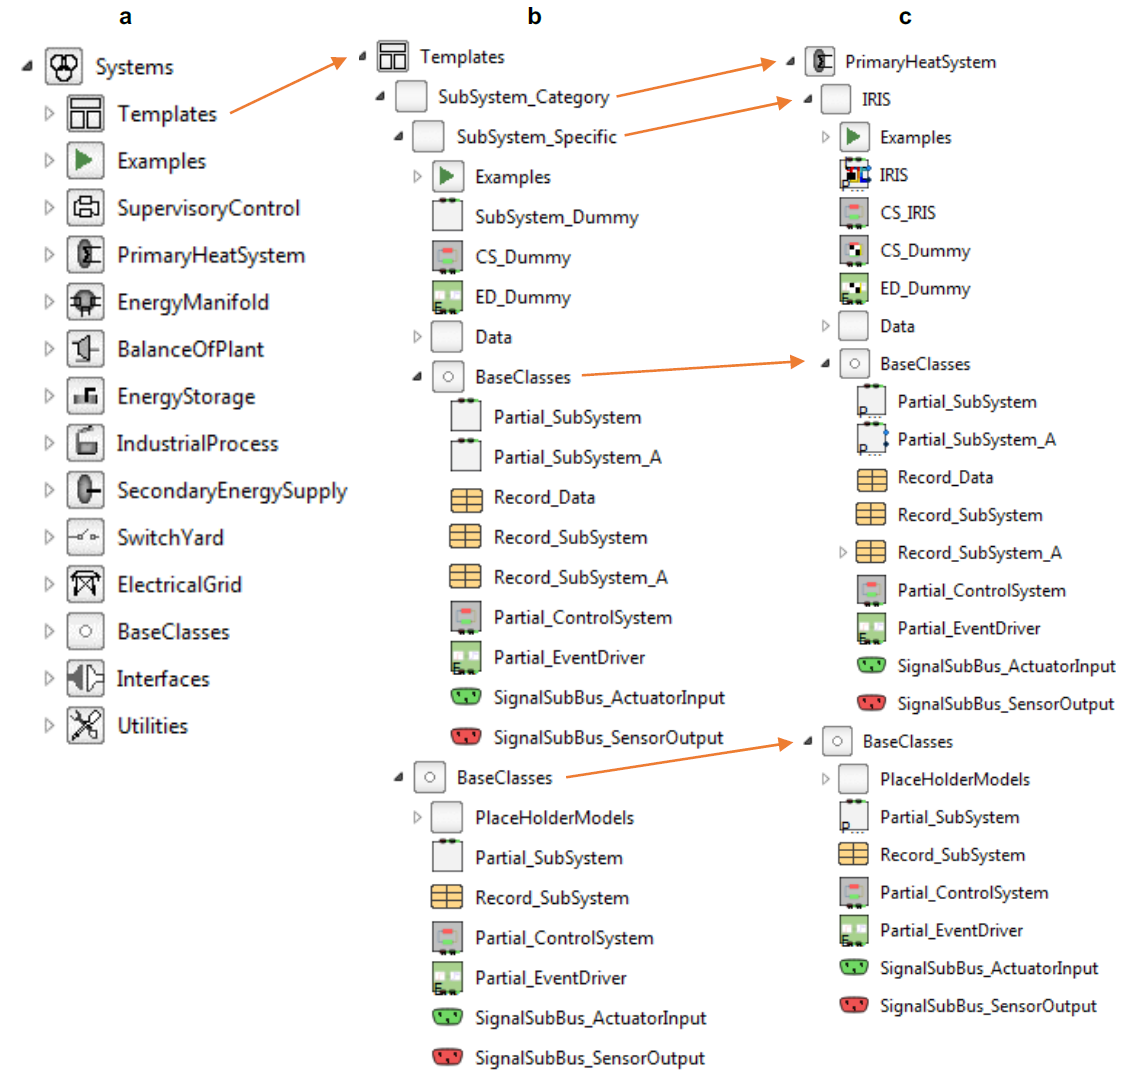
\includegraphics[width=\linewidth]{pics/Template System.png}
\caption{a) Overall Modelica package, b) template structure for creating new subsystem categories and specific subsystem models within a category,  c) example of a specific implementation of a primary heat system using the template approach. }
\label{fig:Template}
\end{figure}



\subsection{Understanding and Running Existing Models}

The hybrid repository is broken down using the templating system shown in Figure \ref{fig:Template}. 
The top level is the overall system package which incorporates all of the Modelica models contained within the NHES package. Then inside of the NHES package are the different subpackages (Systems, Electrical, Thermal, etc…). Within each of the subpackages are further subpackages as seen in the Systems package. Within the Systems package there are further subpackages called \textit{SubSystem Category} (Examples, PrimaryHeatSystem, EnergyStorage, etc…). Then within these SubSystem Categories there is yet another level of subpackage that is called \textit{SubSystem\textunderscore Specific}. Within the \textit{SubSystem\textunderscore Specific} category is where development takes place and potential configurations of the different processes take shape. Inside each SubSystem\textunderscore Specific there is a template that includes \textit{Examples}, \textit{Subsystem Dummy}, \textit{CS\textunderscore Dummy}, \textit{ED\textunderscore Dummy}, Data, BaseClasses, and usually a Components folder. For existing systems the Examples folder contains a runnable example the user can execute to see how the code runs at a top level and what scenarios it is capable of running. An example of which is depicted in Figure \ref{Example File}. For each example the user can double click on the main system which will open the table in the upper left hand corner of Figure \ref{Example File} which provides inputs for the user to change parameters about the system. Then if the user wishes to modify the control system utilized they can either choose from the drop-down menu, or click the button at the right of the “CS” line to open the table in the lower left hand section which provides options to delay when different control systems come online.  

\begin{figure}[hbtp]
\centering
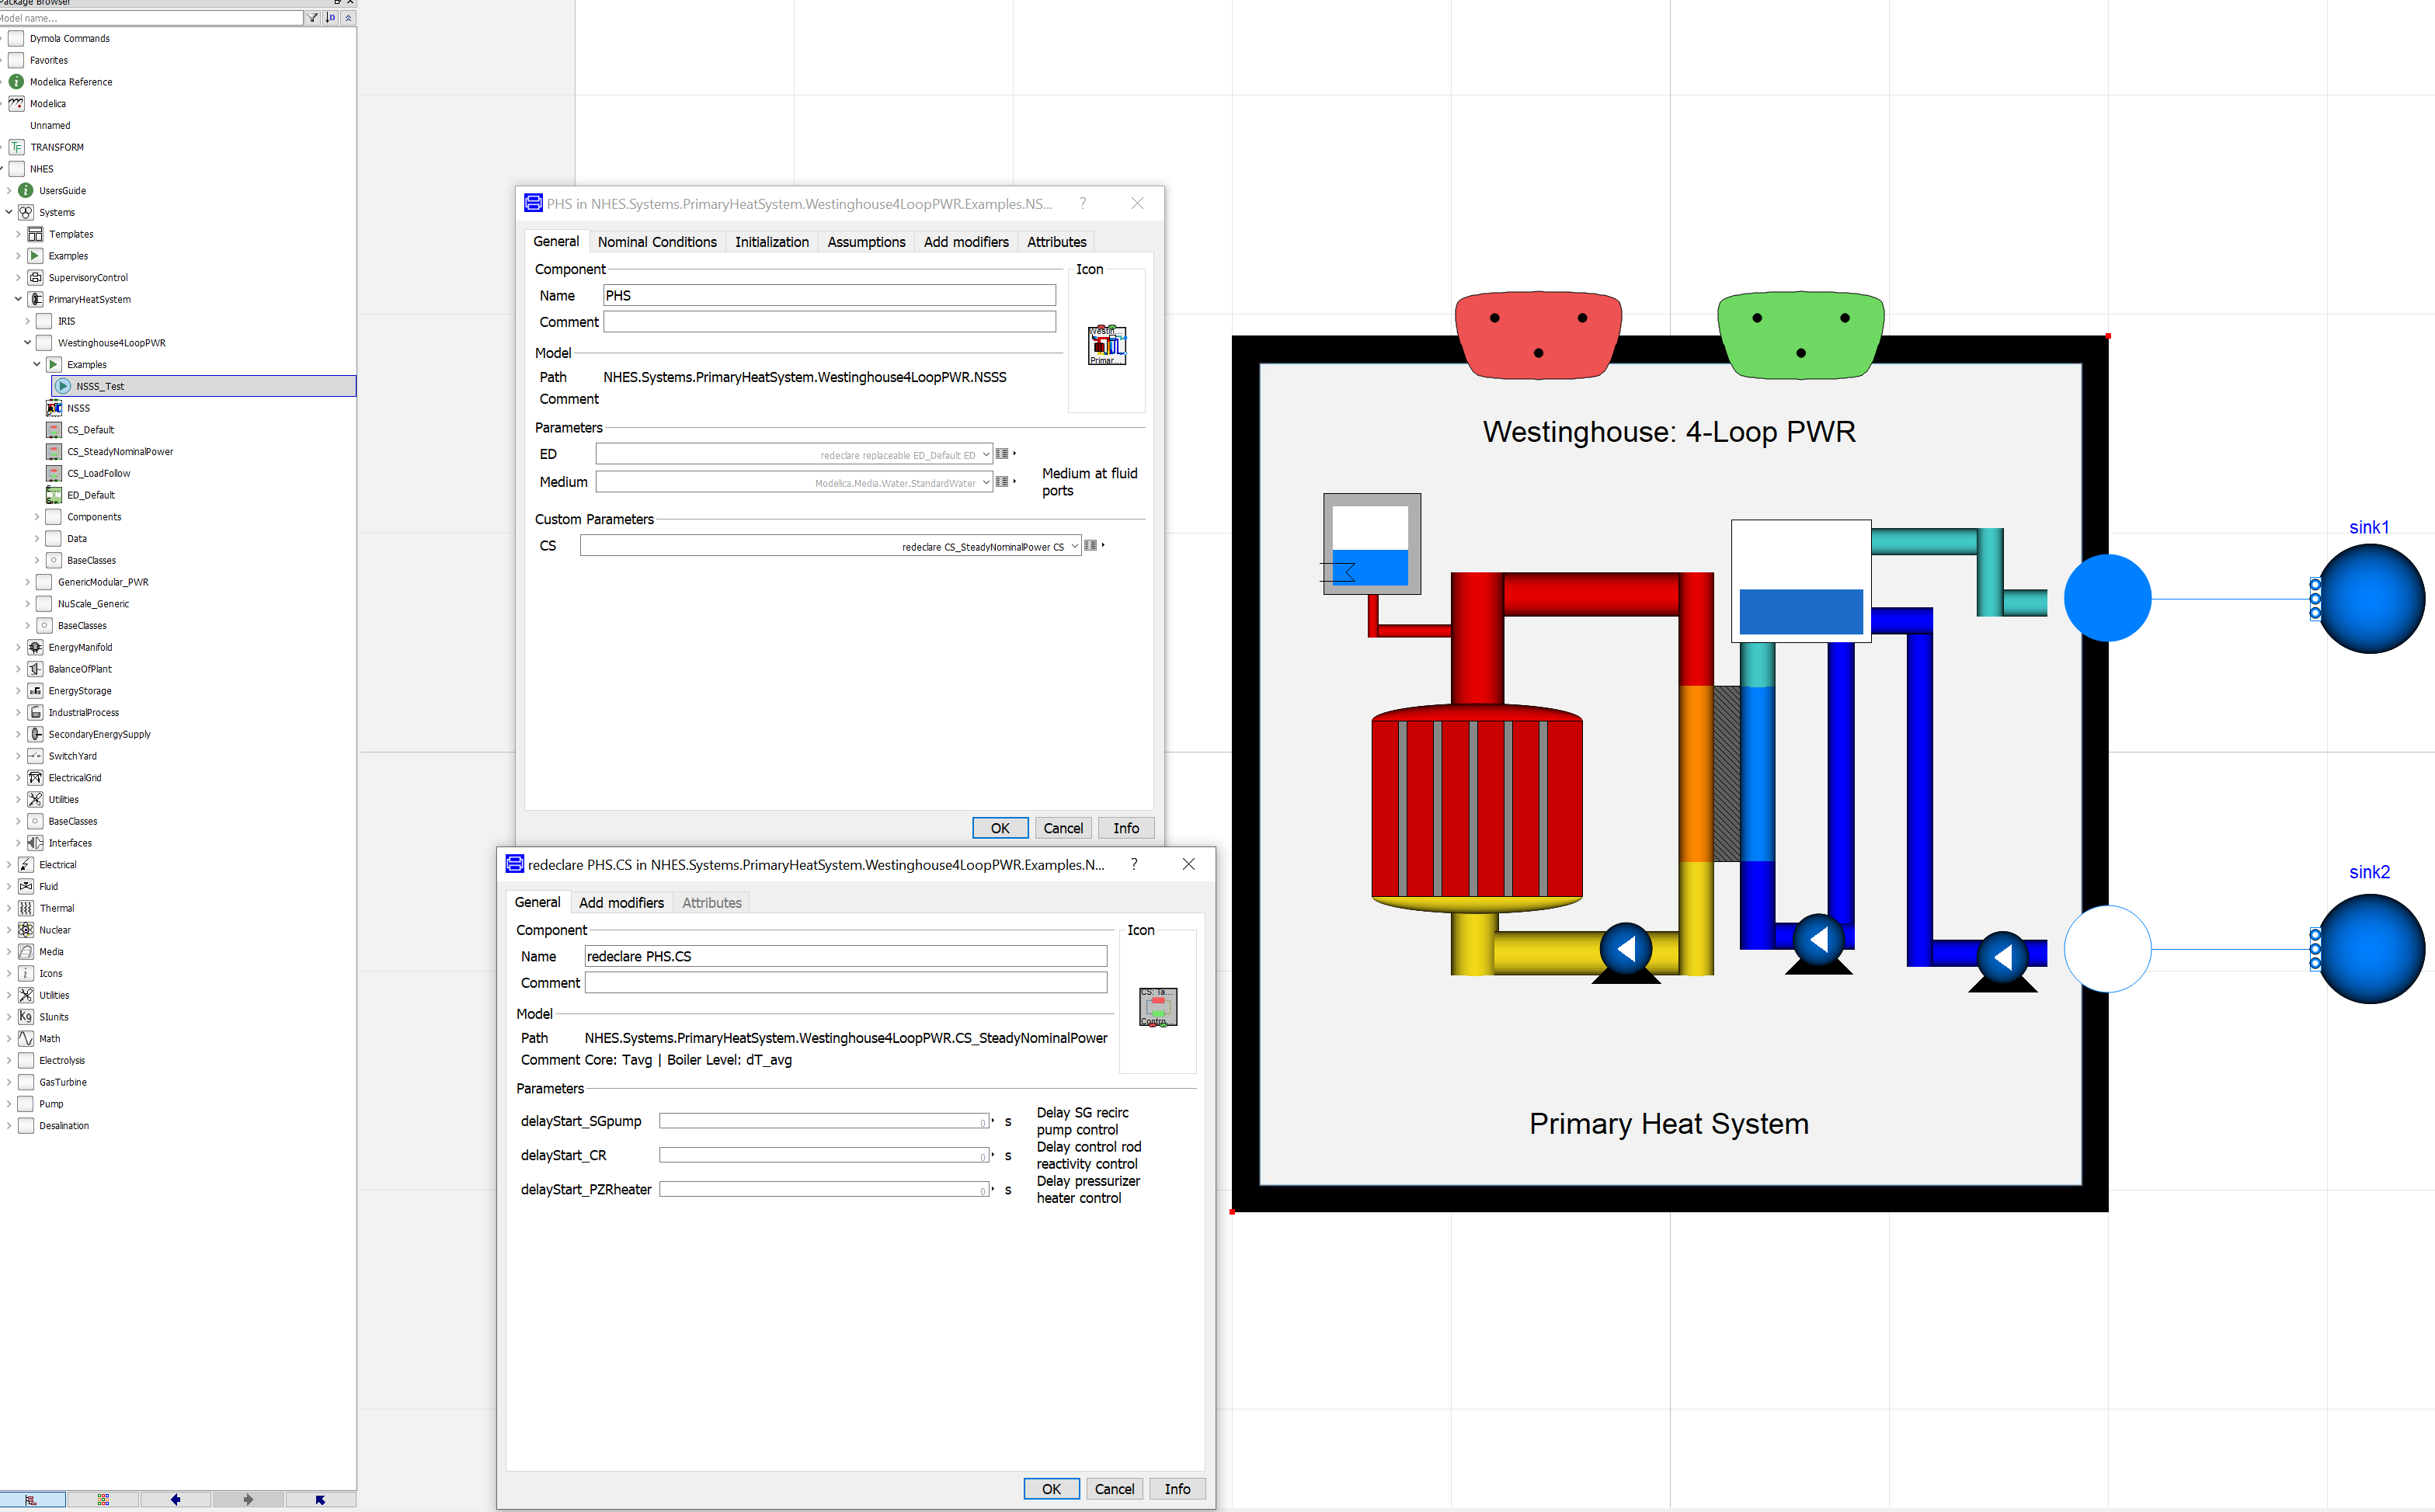
\includegraphics[width=\linewidth]{pics/Example_File.png}
\caption{Exploded view of the NSSS\textunderscore Test example within the NHES library with control system options opened up }
\label{Example File}
\end{figure}

These example tests provide a good way for the user to become associated with the large subsystem in terms of how they work and the different parameters that can be utilized to tune and interact with the models. In addition to the examples file a deeper understanding of the model can be realized by looking into the component structure of the model. This is typically accomplished through looking at the filled-out Subsystem Dummy section. For the Westinghouse 4-Loop plant this can be seen in Figure \ref{Westinghouse 4-loop}. This model includes several subcomponents connected into a singular model. Each model with its’ own set of parameters. Using this version of the model it is possible to discern the inner workings of the model in terms of sensors, physical descriptions of the code, inlet and outlet conditions, and system dependencies. 
In addition to the SubSystem Dummy section, large process models typically include a control system section which is created from the CS\textunderscore Dummy file in the branch. These control system files can be added as a control system for the Subsystem to control different valves, pumps, and control drives within the process from the dropdown menu in the “CS” section seen in Figure \ref{Example File}. large process systems may have several different potential control systems based upon what type of Integrated Energy System they are operating within. An illustration of one of the Westinghouse Control systems can be seen in Figure \ref{Control System}. 


\begin{figure}[hbtp]
\centering
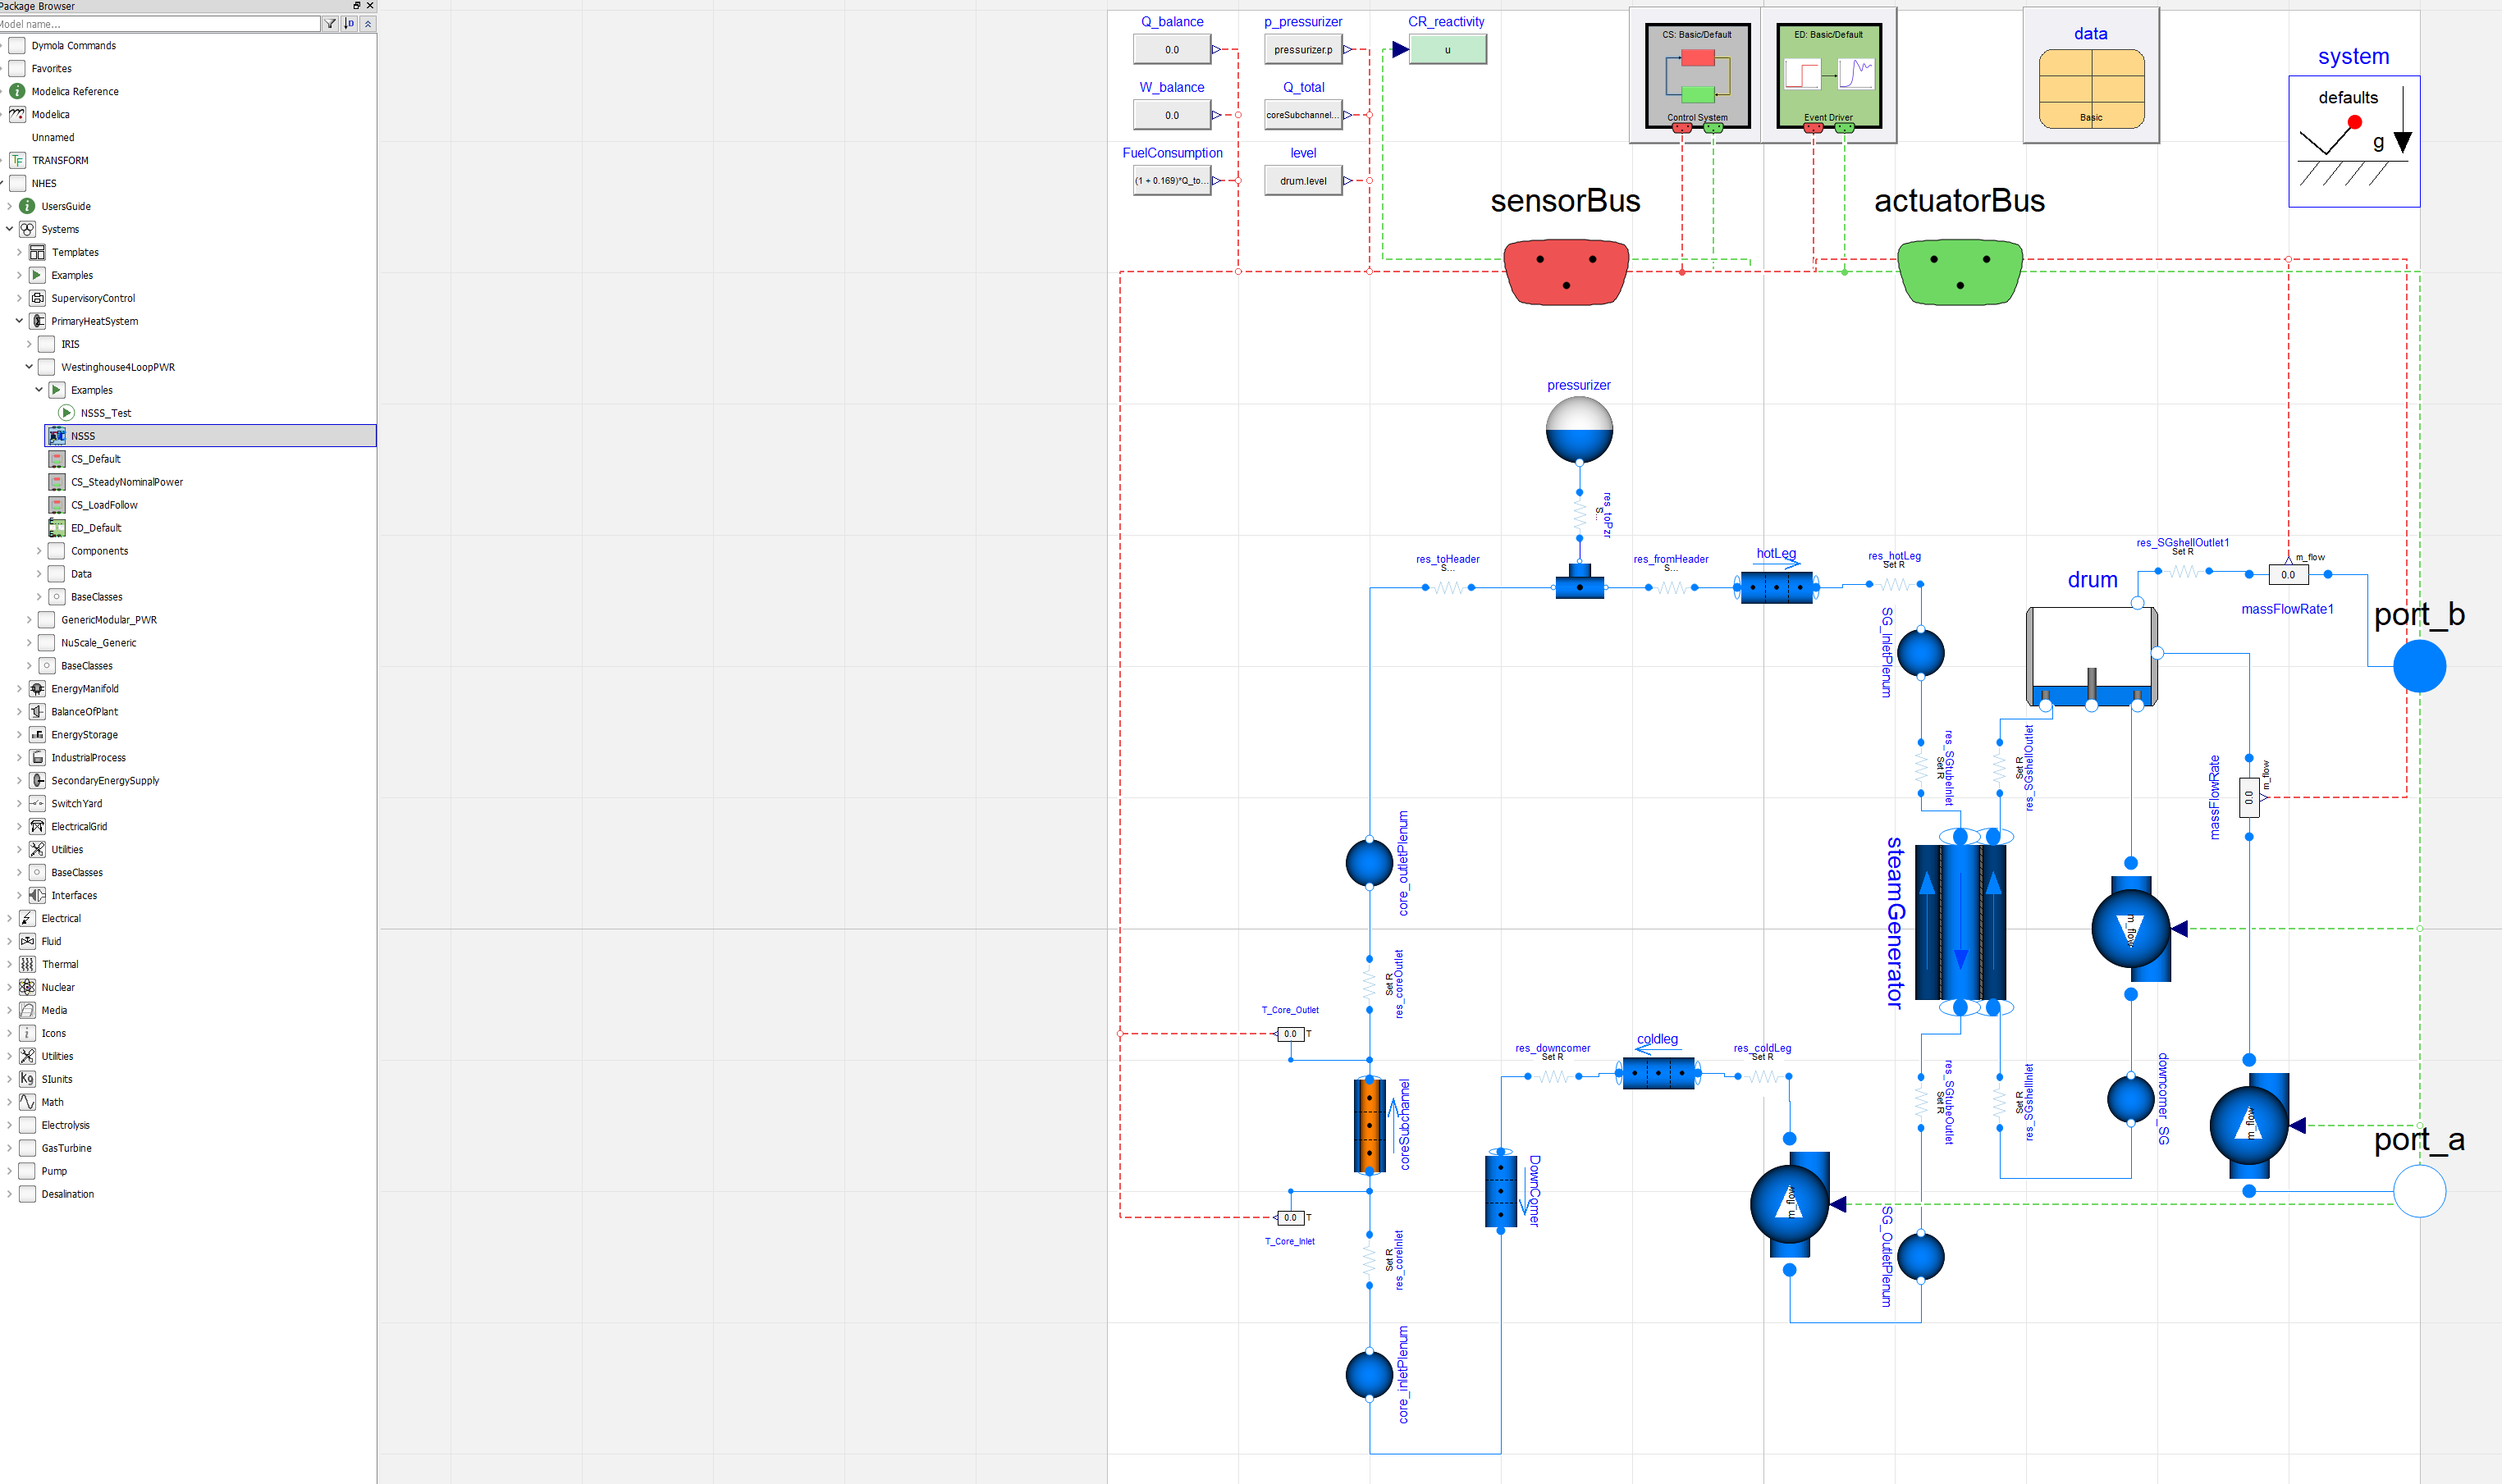
\includegraphics[width=\linewidth]{pics/Sub_System_Dummy.png}
\caption{Subsystem for the Westinghouse-4 Loop model.}
\label{Westinghouse 4-loop}
\end{figure}


\begin{figure}[hbtp]
\centering
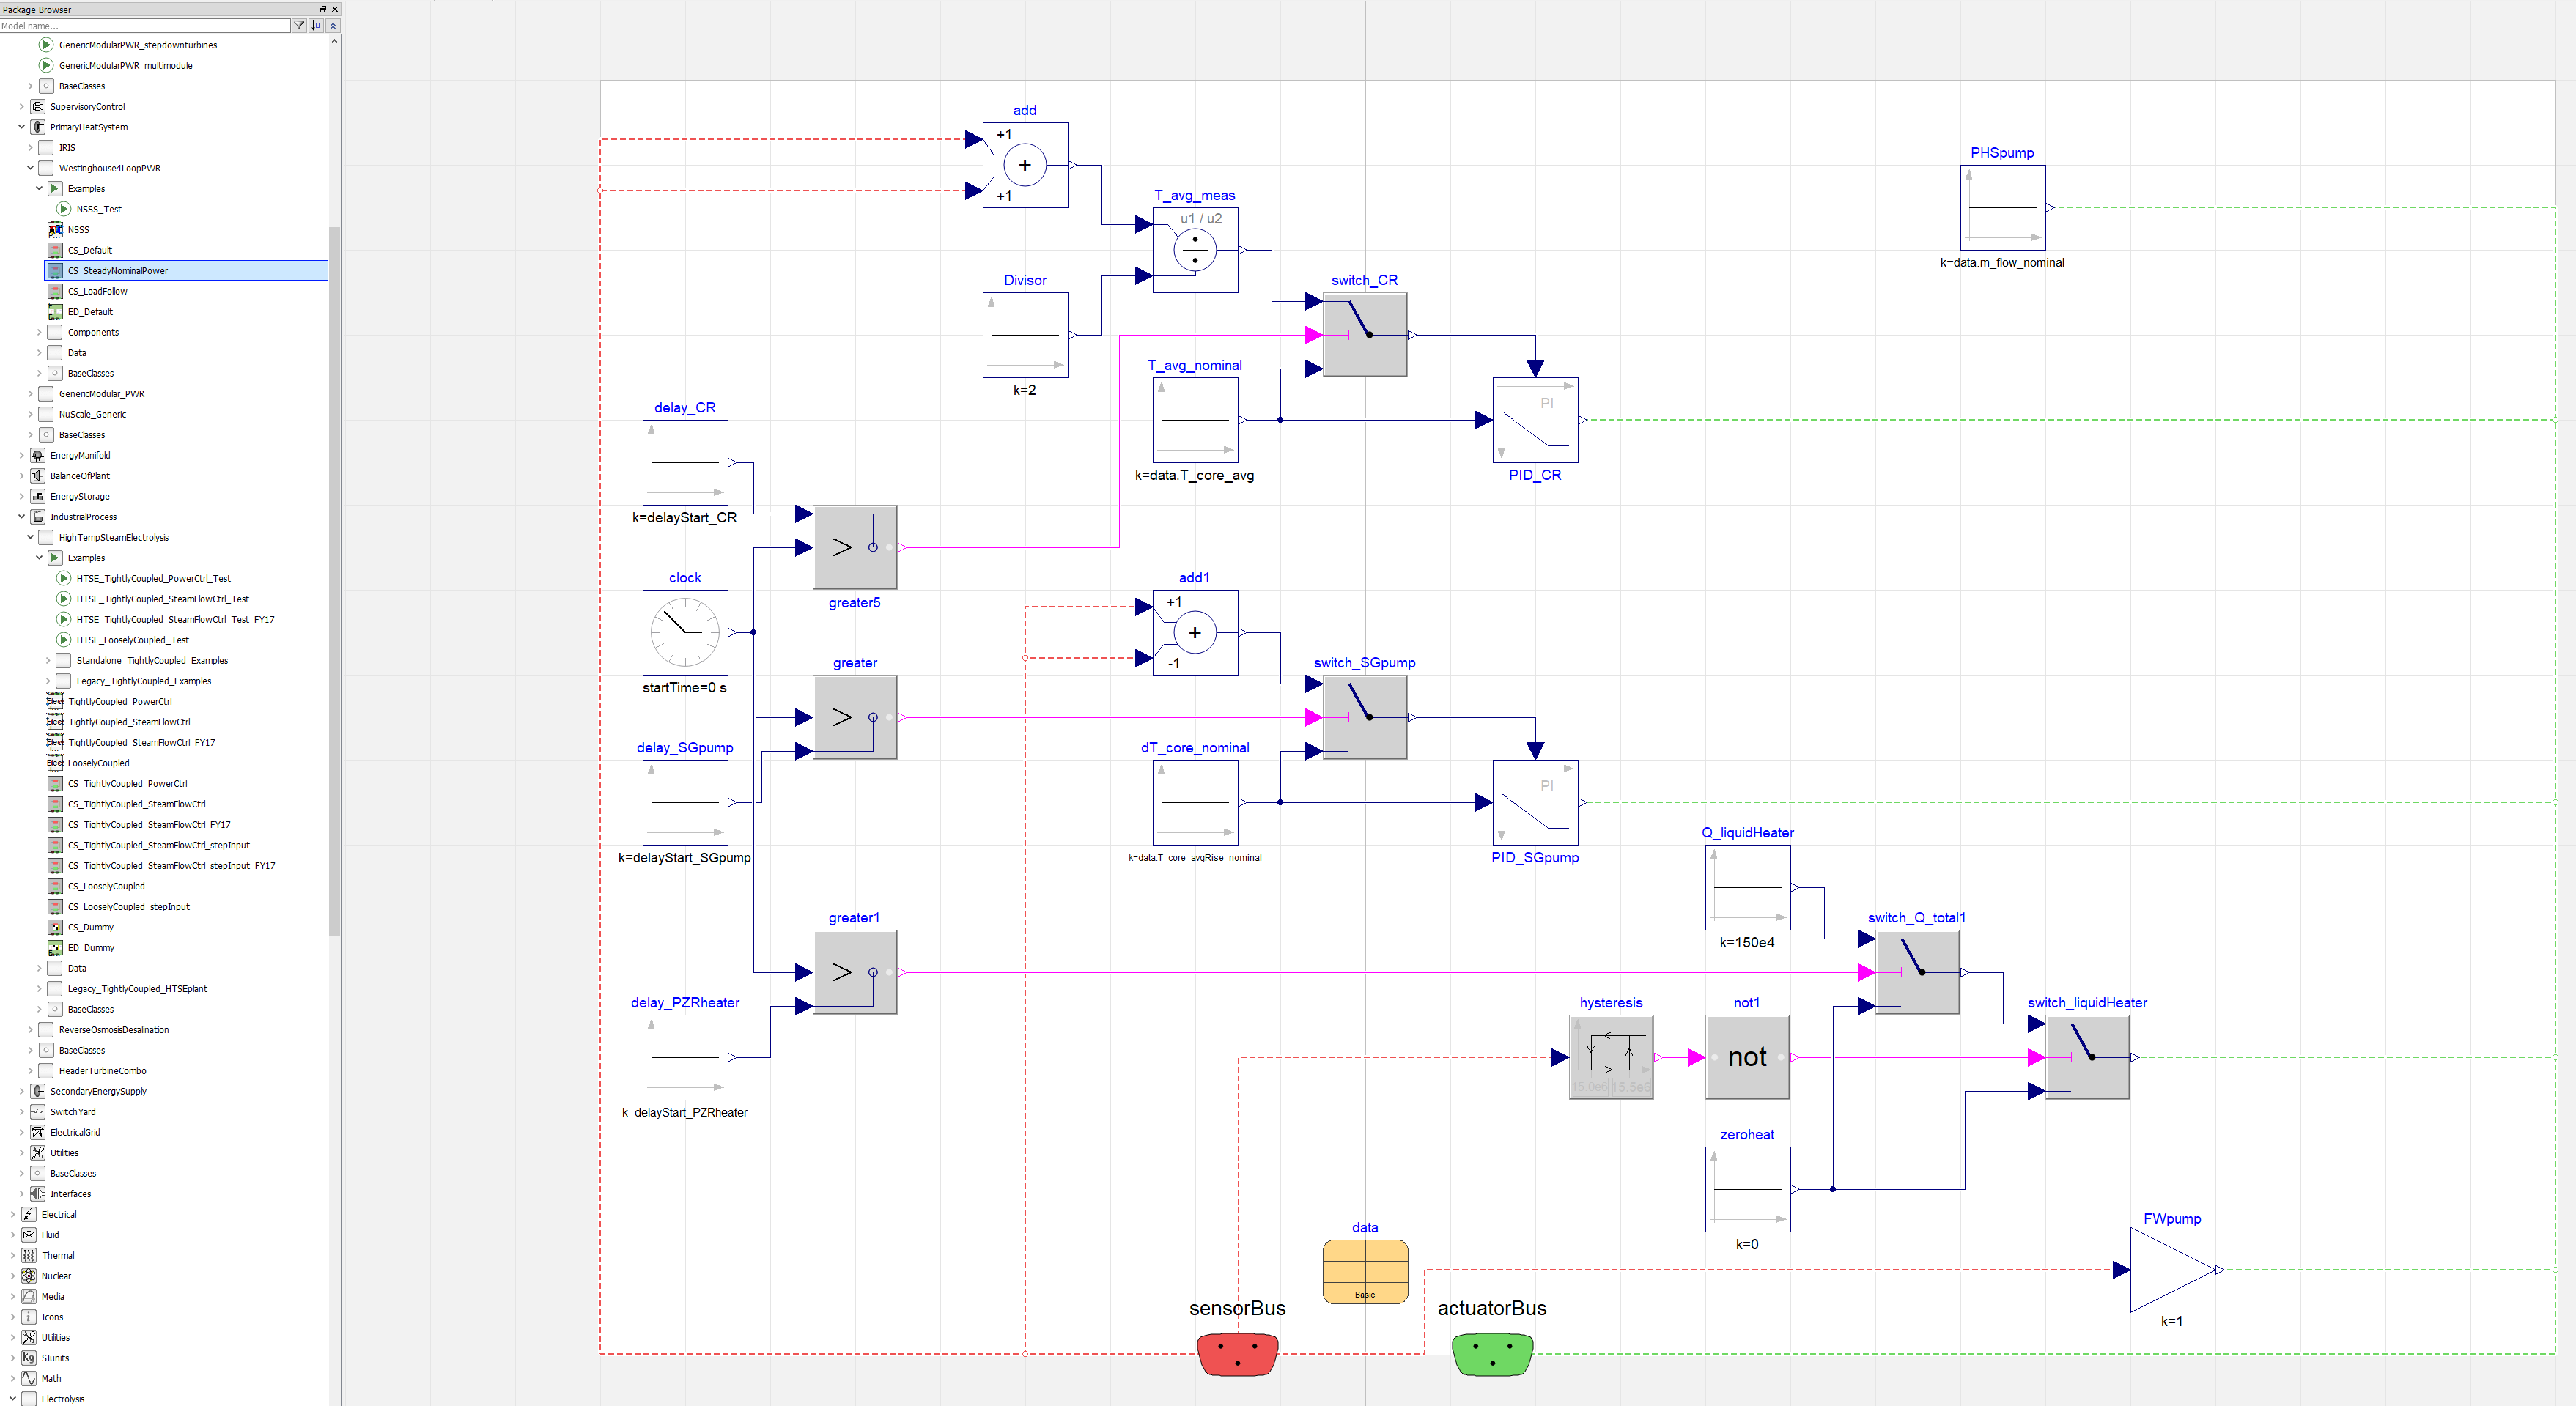
\includegraphics[width=\linewidth]{pics/Westinghouse_Control_picture.png}
\caption{Control System (CS) for the Westinghouse 4 Loop model}
\label{Control System}
\end{figure}

Assuming the user is creating a new package with new components specific to the model it is best to include those models with a “components” folder in the subpackage containing the “BaseClasses” folder. The Data folder is typically where the main data structures in terms of “records” of kept for the process model. Records are files that are intended to be used as an input deck to the main model for use as a set of “parameters” the components will read from. The ED\textunderscore dummy file within the \textit{Subsystem\textunderscore Specific} category is the Event Driver file and is rarely used and can be ignored from a user perspective.

\subsubsection{Modifying Existing Models for Specific Runs}
A starting point from which a user can begin model development and analysis is from an existing Example model. To properly edit the \textit{Examples} within the hybrid repository while still maintaining the regression system one needs to create a duplicate model of the example file that is to be edited. This can be done by right clicking on the file as shown below and creating a duplicate class.

\begin{figure}[hbtp]
\centering
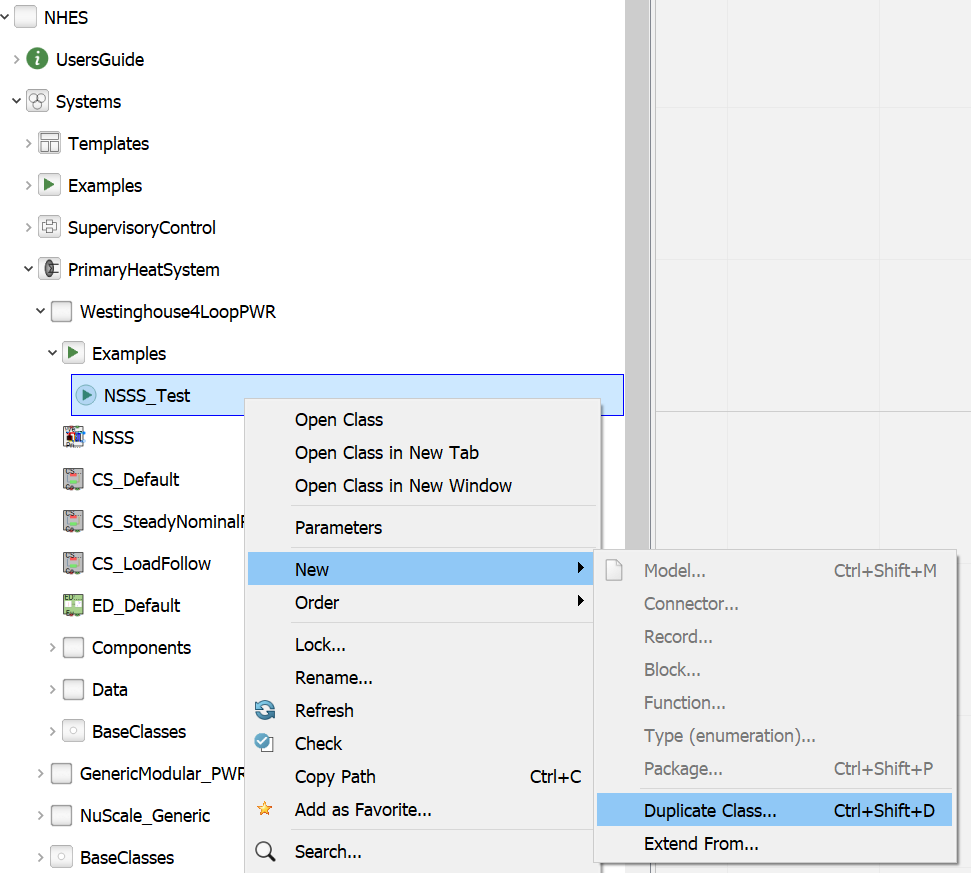
\includegraphics[width=\linewidth]{pics/DuplicateClass.png}
\caption{Creating a duplicate class for model runs.}
\label{Duplicate Class}
\end{figure}

This file will the be placed in the Examples folder where edits can be made to it for new and unique runs. This includes things such as new control schemes, sizing, timeruns, etc..

\subsection{Configuring Existing Models into Integrated Energy Systems}
Each subsystem of the Integrated Energy Systems is inherently interesting on its own and large spans of time can be spent researching and fine tuning them independently. However, the developer team is aware that in the evolving energy landscape, and to the extent users will come across this repository, that integrated energy systems are the primary focus.

This focus includes systems that involve the distribution of heat and electrical energy among several subsystems and the control schemes utilized to accomplish this. Therefore, this section seeks to provide an introductory understanding of how to connect subsystems together within the Hybrid repository. To accomplish this the NuScale\textunderscore Coupling\textunderscore Test Example will be created starting from the GenericModularPWR\textunderscore park system.

\begin{figure}[hbtp]
\centering
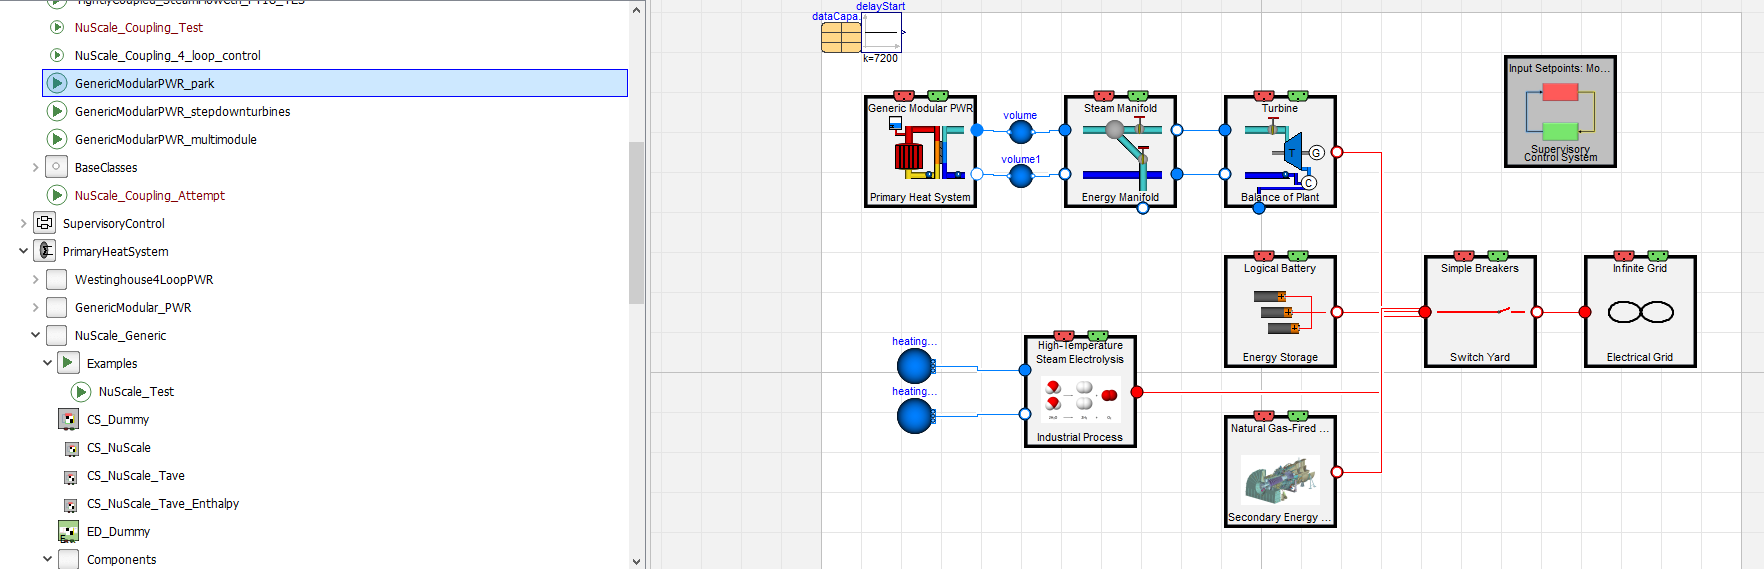
\includegraphics[width=\linewidth]{pics/Modular_Park_Start.png}
\caption{Initial Integrated Energy System Starting Point}
\label{modular park}
\end{figure}

The first step is to take a similar example that has the Supervisory Control System in the top level. In this case the GenericModularPWR\textunderscore park was used. A duplicate class was created and all the components aside the Steam Manifold, Turbine, Simple Breakers, infinite grid, supervisory control system, delay start, and data capacity were removed. See below.

\begin{figure}[hbtp]
\centering
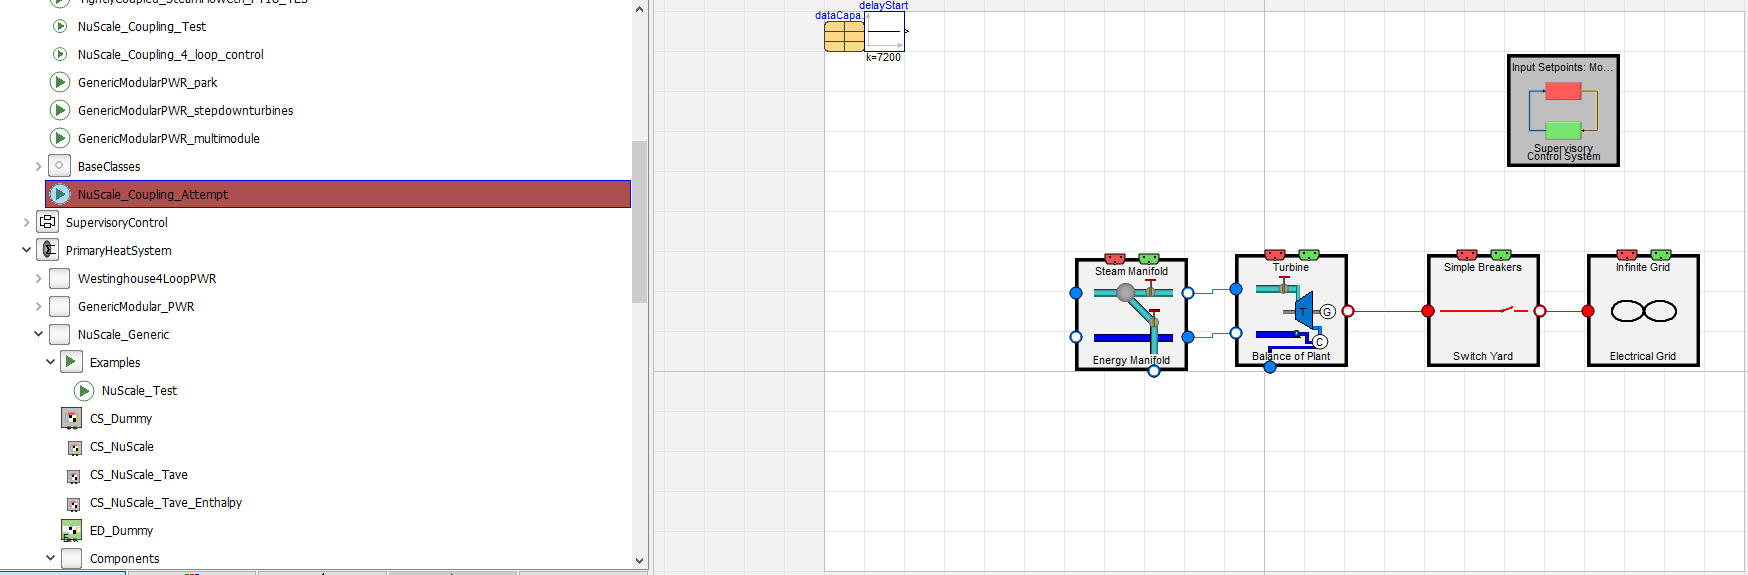
\includegraphics[width=\linewidth]{pics/CouplingCreation.png}
\caption{Rearrangement of Initial Energy System}
\label{coupling park}
\end{figure}

Then the primary side of the NuScale was added in this case the \textit{NuScale\textunderscore Taveprogram} version of the NuScale primary unit.

\begin{figure}[hbtp]
\centering
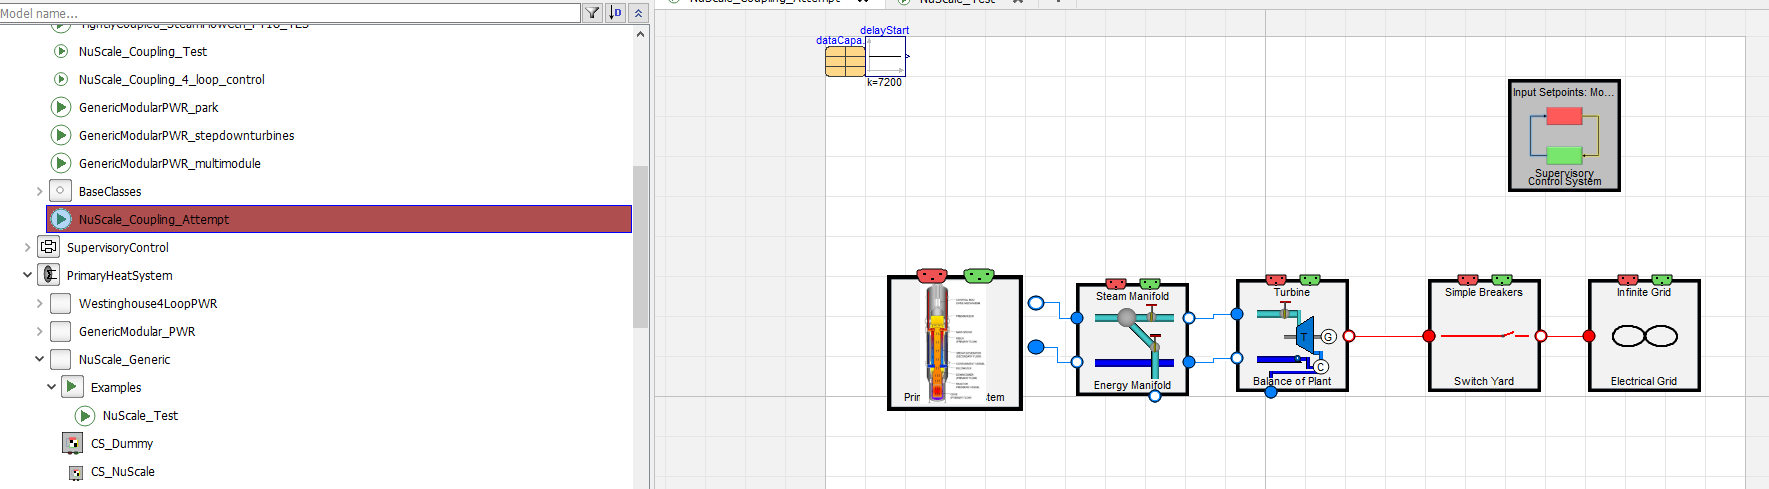
\includegraphics[width=\linewidth]{pics/CouplingCreation_2.png}
\caption{Creation of NuScale Energy System}
\label{NuScale park}
\end{figure}

Then from this point it is a matter of telling the systems what control schemes to use. For this system the reactor operates to meet a certain primary system average temperature in accordance with the turbine output. To input this the control system: PrimaryHeatSystem.NuScaleGeneric.\\ CS\textunderscore NuScale\textunderscore Tave was used with input:
W\textunderscore turbine = BOP.powerSensor.power and W\textunderscore Setpoint  =  SC.W\textunderscore totalSetpoint\textunderscore BOP, see Figure \ref{primary controller settings}.  And the turbine control scheme is modified to reflect a once through system type control strategy where the turbine control valve operates to meet a constant pressure in the turbine, Figure \ref{Turbine Control Settings}. While it is noted that is not the official control strategy strictly speaking for the NuScale system nor is it the one used in load following scenarios in the hybrid repository, it does provide a baseline for which to control the system and modifications can be made from this point.  The power setpoints in the BalanceOfPlant.Turbine.CS\textunderscore OTSG\textunderscore Pressure control module are 160MW for both Reactor\textunderscore Power and Nominal\textunderscore Power while p\textunderscore nominal parameter is set to BOP.port\textunderscore a\textunderscore nominal.p to ensure a single parameter value is carried throughout the system. Additionally, W\textunderscore totalSetpoint is set to SC.W\textunderscore totalSetpoint\textunderscore BOP, Figure \ref{Turbine Control Settings}.

\begin{figure}[hbtp]
\centering
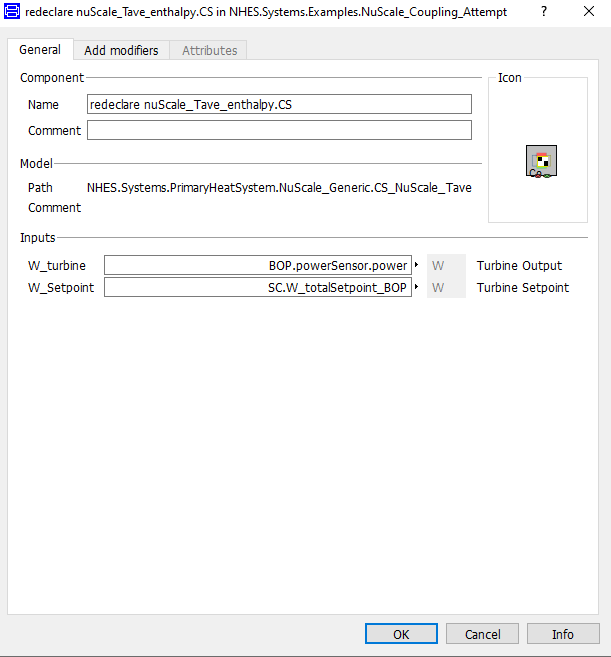
\includegraphics[width=\linewidth]{pics/primary_controller_settings.png}
\caption{Primary System Controller Settings}
\label{primary controller settings}
\end{figure}


\begin{figure}[hbtp]
\centering
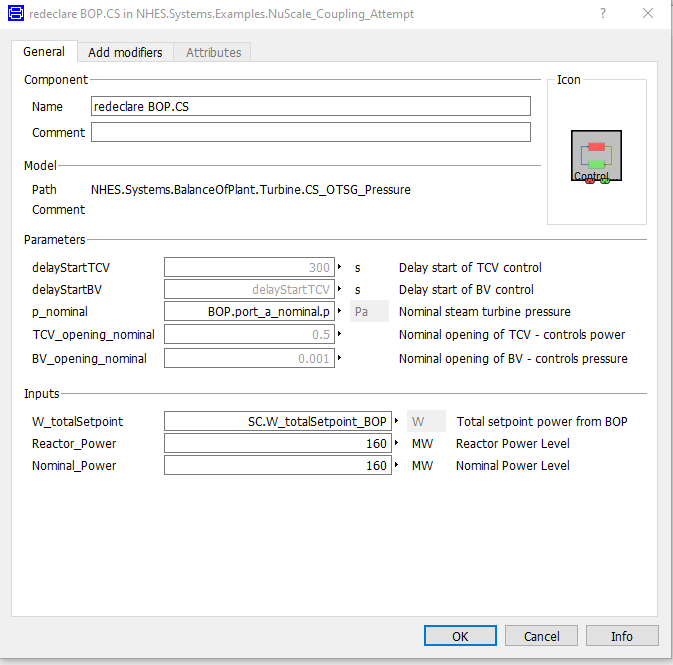
\includegraphics[width=\linewidth]{pics/BOP_settings.png}
\caption{Turbine Control Settings}
\label{Turbine Control Settings}
\end{figure}

To complete the construction of the model the systems need to match on the boundaries.  To do this the values from the primary heat system need to be transferred to the Steam Manifold under the nominal values tab, Figure \ref{Port a Nominal Values} and \ref{port B Nominal Values}.

\begin{figure}[hbtp]
\centering
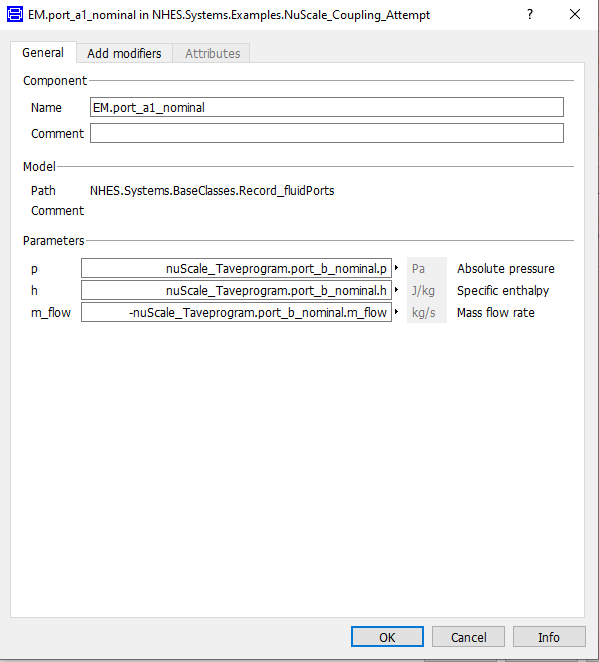
\includegraphics[width=\linewidth]{pics/Nominal_Values_BOP.png}
\caption{Port a Boundary Values of the Energy Manifold}
\label{Port a Nominal Values}
\end{figure}

\begin{figure}[hbtp]
\centering
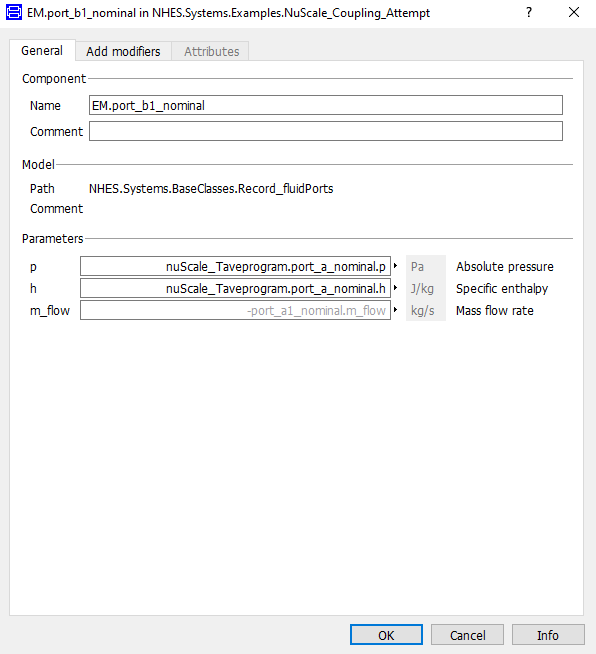
\includegraphics[width=\linewidth]{pics/Manifold_Nominal_b.png}
\caption{Port b Nominal Values of the Energy Manifold }
\label{port B Nominal Values}
\end{figure}

\subsection{Test Creation}
To create a regression test once a user develops an example test in the Dymola NHES library can be accomplished through a couple of settings. In the Dymola simulation setup tab in the output tab uncheck the store at variable events box. Then click store in model button and check the output box, click ok, then click ok again, then Save the model. Example settings are shown in Figure \ref{mat file settings}.


%\begin{figure}[hbtp]
%\caption{dfgsg}
%\centering
%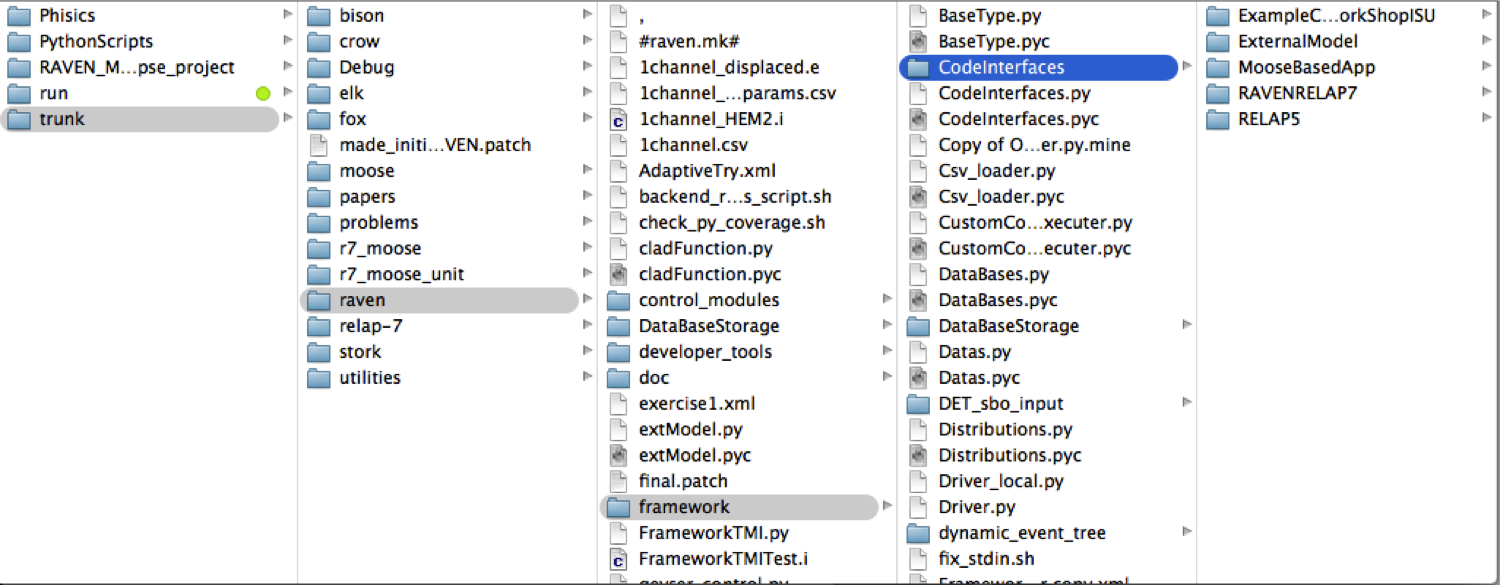
\includegraphics[width=\linewidth]{pics/CodeInterfaceLocation.png}
%\end{figure}


\begin{figure}[hbtp]
\centering
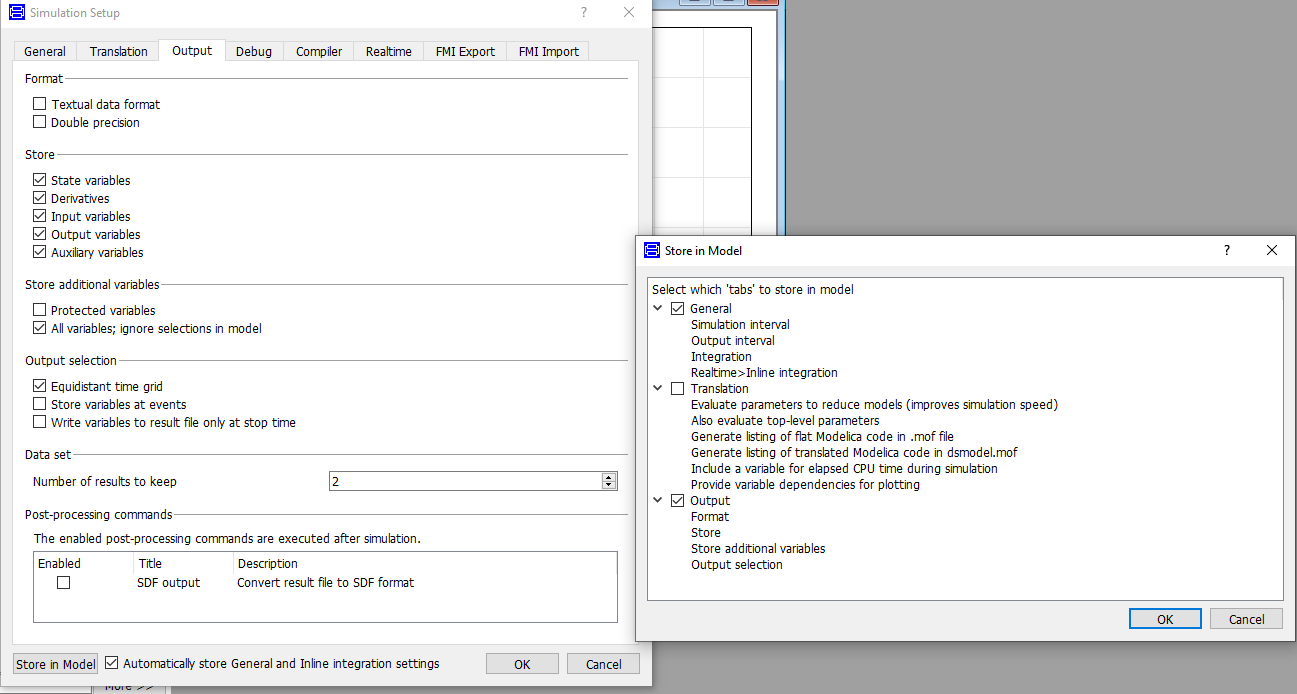
\includegraphics[width=\linewidth]{pics/Test_Creation.png}
\caption{Settings to Create a proper mat file for a gold folder test}
\label{mat file settings}
\end{figure}
In the simulateModel command one of the following two flags is required. Either "\textit{numberOfIntervals}" or "\textit{OutputInterval}". numberOfIntervals tells dymola how many output intervals to make. OutputInterval tells dymola at what timestep interval should an output be present for comparison. The .mat file in the gold folder will need to be run using the same simulateModel command that is present in the .mos file being created.

These can be selected in the Simulation Setup tab of the Dymola GUI, Figure \ref{Interval Setup}, and should carry down to the command you copy and paste in the .mos file. An example is shown below of the simulation setup tab.

\begin{figure}[hbtp]
\centering
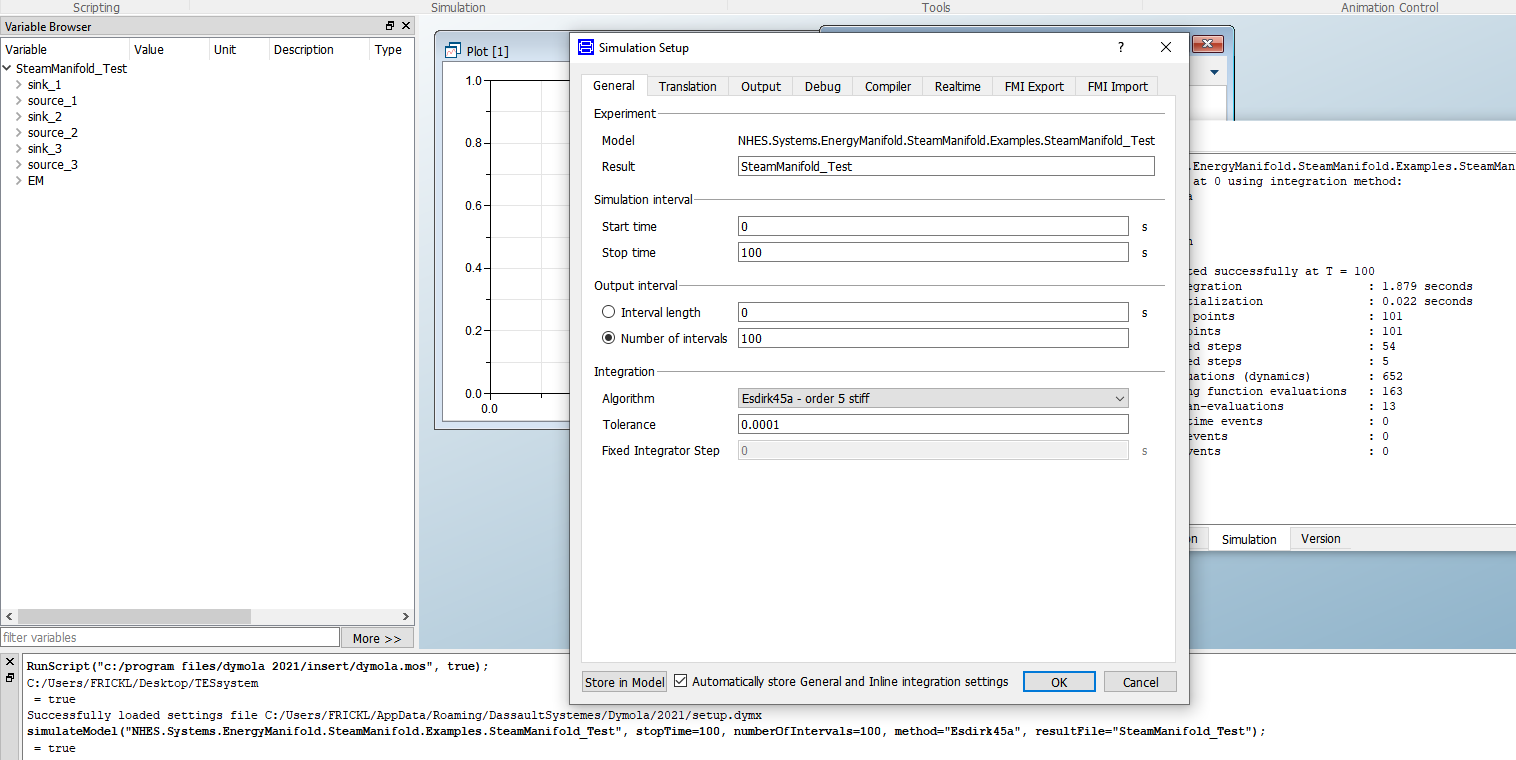
\includegraphics[width=\linewidth]{pics/Regression_picture.png}
\caption{Simulation Setup}
\label{Interval Setup}
\end{figure}

Then run the simulation, (ideally a test should take less than 100 seconds). On the simulation tab in the command line copy the simulation command. Example below:

\begin{lstlisting}[language=bash, basicstyle=\small]
simulateModel("NHES.Systems.EnergyManifold.SteamManifold.
Examples.SteamManifold_Test", stopTime=100, numberOfIntervals=100,
method="Esdirk45a", resultFile="SteamManifold_Test");
\end{lstlisting}

This command should then be added to a file and named something like Test\textunderscore Example.mos. The command can be found in the Simulation Setup tab of the Dymola GUI once you hit simulate

Then in folder /path/to/hybrid/hybrid/tests/dymola\textunderscore tests create a folder named Test\textunderscore YourModel.

Create a \textit{gold} folder in the new folder, drop the .mat file from your simulation that is named resultFile="SteamManifold\textunderscore Test" from your simulateModel command into the gold folder. The .mat file is created in your working directory in Dymola. Then in the main Test\textunderscore YourModel folder drop the Test\textunderscore Example.mos file and create a tests file open it up and place the following in it:


\begin{lstlisting}[language=bash, basicstyle=\small]
[Tests]
 [./]
  type = 'HYBRIDTester'
  input = 'Test_Example.mos'
  workingDir = '.'
  output = 'SteamManifold_Test.mat'
  dymola_mats = 'SteamManifold_Test.mat'  
  rel_err = 0.001
 [../]
[]
\end{lstlisting}

where SteamManifold\textunderscore Test.mat should be your result .mat file name, rel\textunderscore error is the amount of error allowed between the gold file and the regression test output, and Test\textunderscore Example.mos is the run script created.

\subsection{Advanced Test File Options utilized for complex models}
For complex models the initialization phase of a simulation can take the Modelica solvers a significant amount of time to find an initialization point. This occurs due to the highly nonlinear nature of the underlying physical equations.  A way to avoid such situations is to provide a restart file to bypass the initialization phase of the simulation. A restart file is automatically created at the end of each simulation as the dsfin.txt file created in the folder where the simulation is run. This file includes the final values of the previous simulation from which the new model can restart.   Move this file to the gold folder for your new testing system.
Once this file is created it can then be loaded automatically via the continue button in Modelica under the Simulation Tab. Select $Continue \rightarrow  Import Initial  \rightarrow  dsfin.txt  $. See Figure \ref{import Initial}.

\begin{figure}[hbtp]
\centering
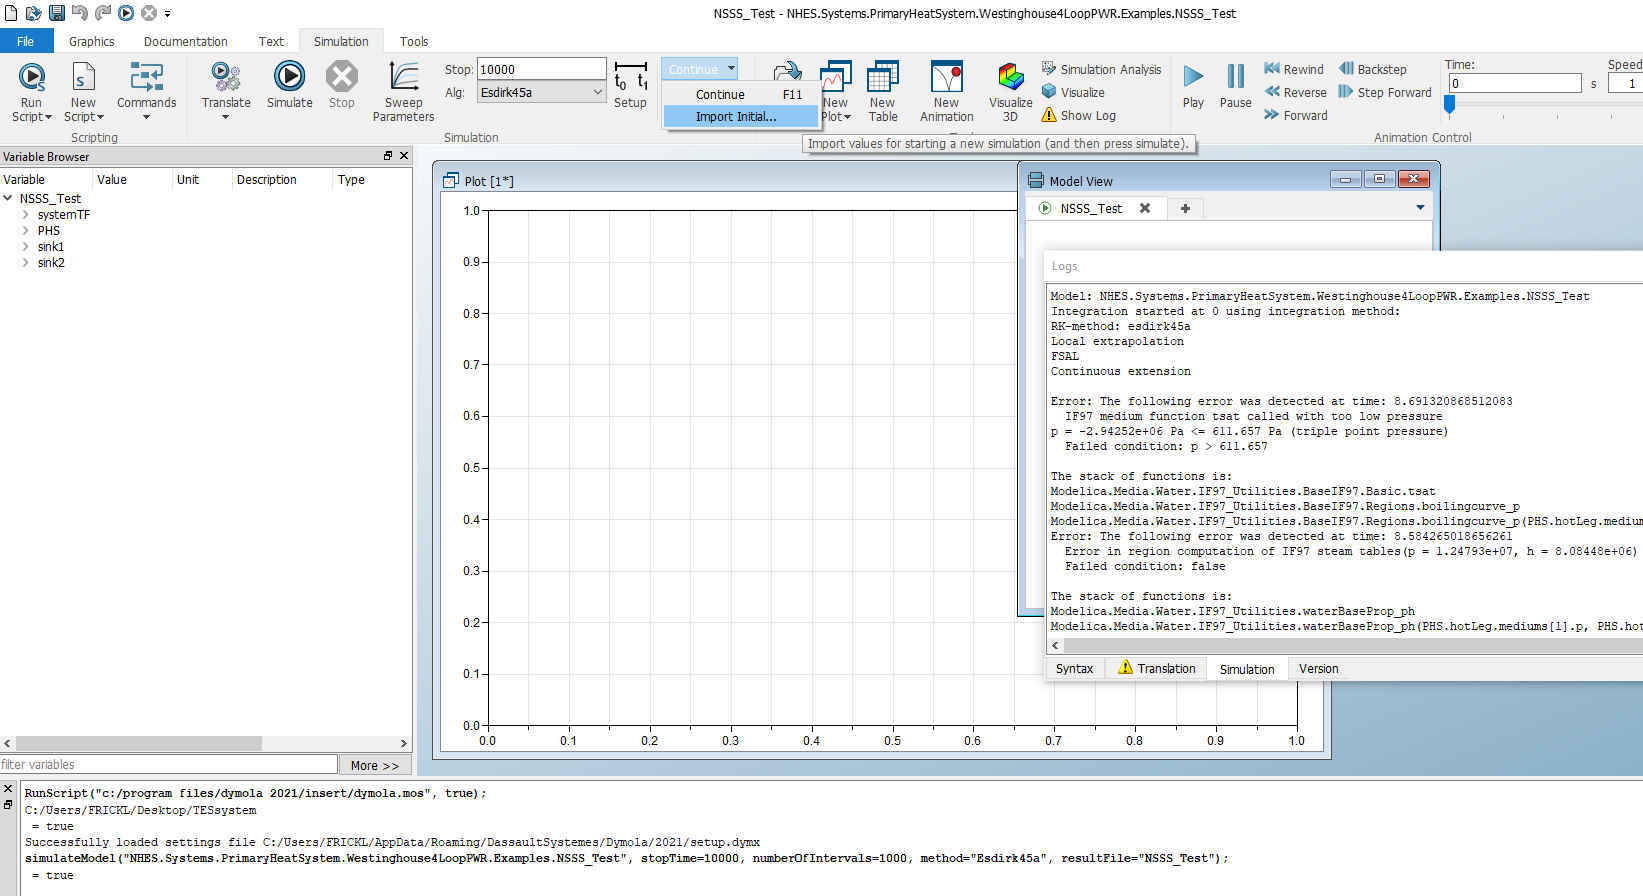
\includegraphics[width=\linewidth]{pics/Import_Initial.png}
\caption{Import Initial conditions from a previously run simulation}
\label{import Initial}
\end{figure}

Then once the dsfin.txt file is loaded go into the Setup tab and move the time back to start from zero and the end time to the desired simulation point for the test, shown in Figure \ref{Simulation Time Realignment}. This is necessary since Dymola assumes the user wants to restart the simulation from where it ended in time as well. This is not the case for the test. Instead the goal is to skip the initialization phase of the simulation and provide a clean solution with which to compare.

\begin{figure}[hbtp]
\centering
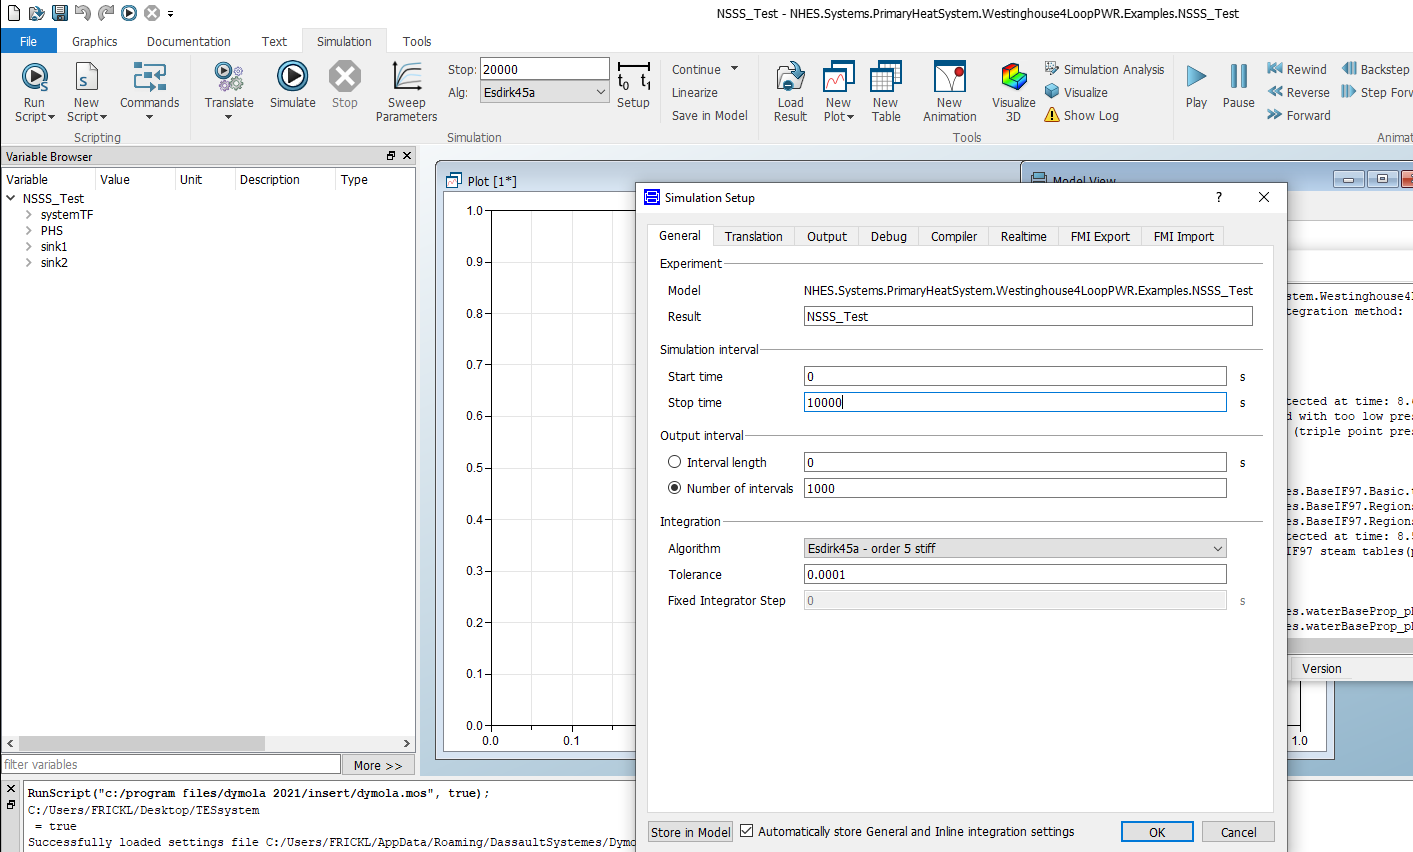
\includegraphics[width=\linewidth]{pics/Move_back_time.png}
\caption{Realign the Simulation Time}
\label{Simulation Time Realignment}
\end{figure}

Simulate this model and save the result file, in this example “NSSS\textunderscore Test.mat” and place it into the gold folder of the testing system. Additionally, copy and paste the simulateModel command that is in the Dymola GUI as the last line of your .mos script file for the test. The first two lines should be translateModel to make sure the right model is loaded into the equation set, followed by the importInitial command that loads all the values into the translated Model. The final command should be the simulateModel command.
The .mos file should look something like what is shown below.

\begin{lstlisting}[language=bash, basicstyle=\small]
translateModel("NHES.Systems.PrimaryHeatSystem.Westinghouse4LoopPWR
.Examples.NSSS_Test");

importInitial("./gold/dsfinal.txt");

simulateModel("NHES.Systems.PrimaryHeatSystem.Westinghouse4LoopPWR.
Examples.NSSS_Test", stopTime=10000, numberOfIntervals=250,
method="Esdirk45a", resultFile="NSSS_Test");
\end{lstlisting}
% definitions

% content
\section{HYBRID Installation Procedure}
\subsection{Overview}

The installation of the HYBRID repository is a straightforward procedure;
depending on the usage purpose and machine architecture, the
installation process slightly differs.

In the following sections, the recommended installation procedure is outlined.  For alternatives, we encourage
checking the \wiki.  The windows 10 machine on which
HYBRID is tested and developed, uses the standard installation procedures outlined below.

The installation process will involve four steps:
\begin{itemize}
  \item Installing prerequisites, which depends on your operating system;
  \item Installing conda;
  \item Installing RAVEN.
  \item Installing HYBRID.
\end{itemize}

\subsection{Cloning the Hybrid Repository}
\label{sec:clone raven}

The first step in installing the package is to clone the HYBRID repository. To do this, use
\begin{lstlisting}[language=bash]
git clone https://github.com/idaholab/HYBRID.git
\end{lstlisting}
This will download the repository into a folder called 'hybrid'. To go inside the folder, use
\begin{lstlisting}[language=bash]
cd hybrid
\end{lstlisting}


\subsubsection{Install RAVEN and its plugins as a sub-module}

The next step is to download and install RAVEN and the submodule (e.g. TEAL, HERON) plugins as a sub-module of the HYBRID repository. 

A submodule allows you to keep another Git repository in a subdirectory of your repository. The other repository has its own history, which does not interfere with the history of the current repository. This can be used to have external dependencies such as third party libraries for example.

In order to get RAVEN do the following in the hybrid folder

\begin{lstlisting}[language=bash]
git checkout devel
\end{lstlisting}

Update the Branch

\begin{lstlisting}[language=bash]
git pull
\end{lstlisting}

to add RAVEN as a submodule
\begin{lstlisting}[language=bash]
git submodule update --init --recursive
\end{lstlisting}

\textbf{Install and Compile RAVEN. }
Once you have downloaded RAVEN as a sub-module, you have to install it. go to the \href{https://github.com/idaholab/raven/wiki/intallationMain}{RAVEN Wiki} for information about how to install it. Run all the tests outlined in the RAVEN wiki. 

\subsubsection{Inform the Framework Paths}

In order to set up the hybrid repository, you must inform the framework about the location of the Dymola python interface. For doing so, navigate to the hybrid directory:

to add RAVEN as a submodule
\begin{lstlisting}[language=bash]
cd <path to your hybrid repository>/hybrid
\end{lstlisting}
Run the following command:
\begin{lstlisting}[language=bash]
./scripts/write_hybridrc.py -p DYMOLA_PATH
\end{lstlisting}

Where DYMOLAPATH is the path to the python interface egg folder in the DYMOLA installation locally. For example:
 
\begin{lstlisting}[language=bash]
./scripts/write_hybridrc.py -p 
	"/c/Program\ Files/Dymola\ 2020x/Modelica/Library/
	python_interface/dymola.egg"
\end{lstlisting}

% definitions
\subsection{Setup of Dymola for the Regression Testing System}
To properly setup the Hybrid repository to work with the regression system one needs to download Dymola as mentioned above and activate the license. Once those two steps are complete the dymola.mos file needs to be edited. The dymola.mos file is the file that tells Dymola what libraries to load when the application is opening and where the working directory is located. For the automatic regression test system to properly test the downloaded library the proper NHES library must be loaded automatically by dymola in the dymola.mos file located at C:/Program Files/Dymola 2020/insert/dymola.mos for example. To properly run the tests the NHES and the TRANSFORM libraries need to be automatically loaded by Dymola upon startup. This can be accomplished by adding to the Dymola.mos until it looks something like:
\begin{lstlisting}[language=python, basicstyle=\small]
RunScript("$DYMOLA/insert/displayunit.mos", true);
definePostProcessing("SDF output", "Convert result file to SDF format", 
"Modelica.Utilities.System.command(\"\\\"%DYMOLA%/bin/dsres2sdf\\\" 
%RESULTFILE%.mat %RESULTFILE%.sdf\")");

openModel("C:\Users\FRICKL\Desktop\TRANSFORM3_20_2020\TRANSFORM- 
Library\TRANSFORM\package.mo"); //Loads Transform package.mo

openModel("C:\msys64\home\FRICKL\hybrid_devel\hybrid\models 
 \NHES\package.mo");//Loads NHES package from hybrid directory
 
cd("C:\Users\FRICKL\Desktop\TESsystem"); 
//Place where all the Dymola runs will occur.
\end{lstlisting}

Having the Dymola.mos file written like this will allow Dymola to automatically load all the needed libraries for Regression testing when conducted using the Regression Test Harness. It should be noted that typically the dymola.mos file will need its permissions to be changed to allow a user to write this. On a Windows machine this is done by running as an administrator on the system and changing the properties of the file to include “read and write” rights, as opposed to “read-only” rights. 

\subsection{Run Regression tests related to the HYBRID project}

Now that the dymola.mos file has been edited to automatically load the TRANSFORM and NHES packages one can run all tests associated with the HYBRID repository. To do this follow the instructions below. 

\begin{lstlisting}[language=bash]
cd <path to your hybrid repository>/hybrid
./run_tests -jX -lY --only-run-types ZZ
\end{lstlisting}
where:
\begin{itemize}
\item "X" is the number of processors to use for testing
\item "Y" is the maximum load to limit to execute tests
\item "ZZ" is the subtype of tests to be run. Currently only "raven" and "dymola" are available.
\end{itemize}

If all tests need to be run, just execute the following command.
\begin{lstlisting}[language=bash]
cd <path to your hybrid repository>/hybrid
./run_tests -jX -lY
\end{lstlisting}
The output will look like the following:

\begin{lstlisting}[language=tex, basicstyle=\tiny ]
######################################################################
#
#  Testing of Hybrid RAVEN Modules  (./run_tests)
#
######################################################################
/c/msys64/home/FRICKL/cleaning_hybrid/hybrid
Found $DYMOLA_PATH and set to C:/Program Files/Dymola 2021/Modelica/Library/python_interface/dymola.egg
Loading raven_libraries conda environment ...
CONDA
... Run Options:
... Mode: 1
... Verbosity: 0
... Clean: 0
... Mode: CONDA
... Conda Defs:
... Loading RAVEN libraries ...
... Detected OS as --os windows ...
... Using Python command python
... $RAVEN_LIBS_NAME set through raven/.ravenrc to raven_libraries
... >> If this is not desired, then remove it from the ravenrc file before running.
... >> RAVEN environment is named "raven_libraries"
... found conda path in ravenrc: C:/Users/FRICKL/AppData/Local/Continuum/miniconda3/etc/profile.d/conda.sh
... >> If this is not the desirable path, rerun with argument --conda-defs [path] or remove the entry from raven/.ravenrc file.
... Found conda definitions at C:/Users/FRICKL/AppData/Local/Continuum/miniconda3/etc/profile.d/conda.sh
conda 4.8.3
raven_libraries          C:\Users\FRICKL\AppData\Local\Continuum\miniconda3\envs\raven_libraries
... Found library environment ...
... Activating environment ...
... Activating environment ...
... done!
rook: loading init file "C:/msys64/home/FRICKL/cleaning_hybrid/hybrid/scripts/rook.ini"
rook: ... loaded setting "add_non_default_run_types = dymola,raven"
rook: ... loaded setting "add_run_types = dymola,raven"
rook: ... loaded setting "test_dir = tests"
rook: ... loaded setting "testers_dirs = scripts/testers,raven/scripts/TestHarness/testers/"
rook: found 27 test dirs under "tests" ...
rook: loading init file "C:/msys64/home/FRICKL/cleaning_hybrid/hybrid/scripts/rook.ini"
rook: ... loaded setting "add_non_default_run_types = dymola,raven"
rook: ... loaded setting "add_run_types = dymola,raven"
rook: ... loaded setting "test_dir = tests"
rook: ... loaded setting "testers_dirs = scripts/testers,raven/scripts/TestHarness/testers/"
(1/27) Success( 40.44sec)tests\dymola_tests\BOP_L1_Boundaries_a_Test\
(2/27) Success( 41.22sec)tests\dymola_tests\BOP_L1_Boundaries_b_Test\
(3/27) Success( 15.27sec)tests\dymola_tests\Desalination_1_pass\
(4/27) Success( 15.84sec)tests\dymola_tests\Desalination_2pass_mixing\
(5/27) Success( 14.17sec)tests\dymola_tests\Desalination_2_pass\
(6/27) Success( 24.64sec)tests\dymola_tests\Desalination_NHES_basic\
(7/27) Success( 22.12sec)tests\dymola_tests\Desalination_ROmodule\
(8/27) Success( 42.10sec)tests\dymola_tests\Desalination_NHES_complex\
(9/27) Success( 17.21sec)tests\dymola_tests\GTTP_Test\
(10/27) Success( 36.21sec)tests\dymola_tests\Generic_Modular_PWR\
(11/27) Success( 23.93sec)tests\dymola_tests\HTSE_Power_Test\
(12/27) Success( 32.00sec)tests\dymola_tests\HTSE_Steam_Test\
(13/27) Success( 39.60sec)tests\dymola_tests\NSSS_test\
(14/27) Success( 55.31sec)tests\dymola_tests\NuScale_4Loop\
(15/27) Success( 36.51sec)tests\dymola_tests\NuScale_Nominal_Test\
(16/27) Success( 15.14sec)tests\dymola_tests\Simple_Breakers_Test\
(17/27) Success( 26.16sec)tests\dymola_tests\NuScale_primary_test\
(18/27) Success( 15.70sec)tests\dymola_tests\StepDownTurbines\
(19/27) Success( 16.61sec)tests\dymola_tests\StepDownTurbines_complex\
(20/27) Success( 14.34sec)tests\dymola_tests\Supervisory_Control_Test\
(21/27) Success( 14.31sec)tests\dymola_tests\Test_Battery_Storage\
(22/27) Success( 34.01sec)tests\dymola_tests\Test_Thermal_Storage\
(23/27) Success( 37.58sec)tests\dymola_tests\Thermocline_Cycling\
"failing"
(24/27) Skipped(  None!  )tests\dymola_tests\TightlyCoupled_FY18_Battery\
"failing"
(25/27) Skipped(  None!  )tests\dymola_tests\TightlyCoupled_FY18_TES\
(26/27) Success( 25.44sec)tests\dymola_tests\Thermocline_Insulation\
(27/27) Success( 31.37sec)tests\raven_tests\train\TrainArmaOnData

PASSED: 25
SKIPPED: 2
FAILED: 0
\end{lstlisting}


%\subsection{Microsoft Windows}
\label{sec:install windows}

The process of establishing the required environment for Windows is notably more involved than the other two
systems; however, it is straightforward.  First, RAVEN has the following prerequisites on Windows:

\begin{itemize}
    \item A system running a 64-bit version of Microsoft Windows. Installation and operation
        has been verified on Windows 7, 10, and Windows Server 2012 R2 Standard.
    \item At least 9 Gigabytes of available disk space:
    \begin{itemize}
        \item 0.5 GB for GIT SCM, including supporting tools and git source code control
        \item 1.5 GB for Python language and supporting packages
        \item 1 GB for RAVEN framework
        \item 5.0 GB for the Visual Studio compiler needed to build RAVEN
    \end{itemize}
\end{itemize}

\subsubsection{A Visual Guide}
Note: An illustrated version of this procedure may be found on the \wiki.

\subsubsection{GIT SCM for Windows}
RAVEN currently works on Windows using basic tools freely available online. 
The first software to be downloaded and installed is \textbf{Git SCM} available at \url{https://gitforwindows.org/}.
\begin{enumerate}
    \item Obtain the latest Git SCM for Windows installer from  \url{https://gitforwindows.org/} and install it. 
    Install Git Bash and have 
    the installer add Git Bash to your Windows \textit{PATH} environment variables. 
    The \textit{PATH} can be updated either automatically (allowing the Git SCM installer to update it for you) or manually 
    (Systems Properties - Environment Variables - Edit Environment Variables).
\end{enumerate}

\subsubsection{Install Python Language and Package Support}
\begin{enumerate}
	\item Download the latest 64-bit installer for Windows Python 3 from
		\url{https://conda.io/miniconda.html} and install it.  \item The installer
		will ask whether Python should be installed for only the logged in user or
		for all users.  Either option will work for RAVEN.
	\item 	have  the installer add \textit{conda} to your Windows \textit{PATH} environment variables.   
	The \textit{PATH} can be updated either automatically (allowing the  \textit{conda} installer to update it for you) 
	or manually (Systems Properties - Environment Variables - Edit Environment Variables).
	\item Check the installation of Python and coda locating and testing the Python installation.   
	Open a Windows command prompt and enter the
		command "{\it where python}", which attempts to locate a the Python language interpreter
		in the current system path.  This looks like:

    \begin{lstlisting}[language=bash, basicstyle=\small]
    C:\Users\USERID> where python
    C:\Users\USERID\AppData\Local\Continuum\Miniconda3\python.exe
    \end{lstlisting}

\end{enumerate}


\subsubsection{Compiler Installation and Configuration}
\begin{enumerate}
	\item Download and install Visual Studio.  A C++ language compiler that supports C++11 features
		is needed to perform this step. Microsoft's Visual Studio Community Edition is free and
		available from \url{https://www.visualstudio.com/downloads/}.

		The current version (as of this writing) is 2017. The 2015 and 2017 versions have been
		successfully used to build RAVEN. Professional and Enterprise versions of these will
		also work. If one of these is already present on your system, it is not necessary to
		obtain another one. Note that because C++11 language features are required, the
		"Microsoft Visual C++ Compiler for Python 2.7 or 3.x" often used for building Python
		add-ons will {\bf not} work.

		After downloading and running the Visual Studio installer, it will ask what features
		to install. For building RAVEN, "Desktop development with C++" is needed at a minimum.
		Installation of other Visual Studio features should be fine.
\end{enumerate}

Once the compiler installation and configuration is complete, you are prepared to install the RAVEN libraries
(see section \ref{sec:install conda}).



%\subsection{Conda: Python Dependencies}
\label{sec:install conda}

The standard installation procedure for RAVEN includes using Miniconda (often simply referred to as
\emph{conda}) to install the Python libraries required to run RAVEN.  If conda cannot be made available on an
operating system, refer to the wiki (listed above) for alternatives.  To install miniconda, follow the
instructions for your operating system at \url{https://conda.io/miniconda.html}.

\nb RAVEN currently works with Python 2.7, but it is recommended that Python 3 be used, so unless you have a reason to use 2.7, we recommend installing the 64 bit Python 3 version of miniconda.

Once conda is installed, proceed to installing RAVEN itself (section \ref{sec:clone raven}).

%\subsection{Cloning the Hybrid Repository}
\label{sec:clone raven}

The first step in installing the package is to clone the HYBRID repository. To do this, use
\begin{lstlisting}[language=bash]
git clone https://github.com/idaholab/HYBRID.git
\end{lstlisting}
This will download the repository into a folder called 'hybrid'. To go inside the folder, use
\begin{lstlisting}[language=bash]
cd hybrid
\end{lstlisting}


\subsubsection{Install RAVEN and its plugins as a sub-module}

The next step is to download and install RAVEN and the submodule (e.g. TEAL, HERON) plugins as a sub-module of the HYBRID repository. 

A submodule allows you to keep another Git repository in a subdirectory of your repository. The other repository has its own history, which does not interfere with the history of the current repository. This can be used to have external dependencies such as third party libraries for example.

In order to get RAVEN do the following in the hybrid folder

\begin{lstlisting}[language=bash]
git checkout devel
\end{lstlisting}

Update the Branch

\begin{lstlisting}[language=bash]
git pull
\end{lstlisting}

to add RAVEN as a submodule
\begin{lstlisting}[language=bash]
git submodule update --init --recursive
\end{lstlisting}

\textbf{Install and Compile RAVEN. }
Once you have downloaded RAVEN as a sub-module, you have to install it. go to the \href{https://github.com/idaholab/raven/wiki/intallationMain}{RAVEN Wiki} for information about how to install it. Run all the tests outlined in the RAVEN wiki. 

\subsubsection{Inform the Framework Paths}

In order to set up the hybrid repository, you must inform the framework about the location of the Dymola python interface. For doing so, navigate to the hybrid directory:

to add RAVEN as a submodule
\begin{lstlisting}[language=bash]
cd <path to your hybrid repository>/hybrid
\end{lstlisting}
Run the following command:
\begin{lstlisting}[language=bash]
./scripts/write_hybridrc.py -p DYMOLA_PATH
\end{lstlisting}

Where DYMOLAPATH is the path to the python interface egg folder in the DYMOLA installation locally. For example:
 
\begin{lstlisting}[language=bash]
./scripts/write_hybridrc.py -p 
	"/c/Program\ Files/Dymola\ 2020x/Modelica/Library/
	python_interface/dymola.egg"
\end{lstlisting}


%\section{Running HYBRID}
\label{HowToRun}

% I don't think this is mentioned earlier? Andrea answers :D It mentioned in the Introduction
%As already mentioned,
The hybrid code is a blend of C++, C, and Python, Modelica languages. The entry point
resides on the Python side and is accessible via a command line interface.
%
After following the instructions in the previous Section, RAVEN is ready to be
used.
%
The \texttt{raven\_framework} script is in the raven folder.
%
To run RAVEN, open a terminal and use the following command (replace \texttt{<inputFileName.xml>} with your RAVEN input file):

\begin{itemize}

  \item \textbf{Any unix-based systems (e.g. Macintosh, Linux, etc.)}:
\begin{lstlisting}[language=bash]
raven_framework <inputFileName.xml>
\end{lstlisting}
  \item \textbf{Windows}:
  \begin{lstlisting}[language=bash]
bash.exe raven_framework <inputFileName.xml>
\end{lstlisting}
  
\end{itemize}

Using \texttt{raven\_framework} is the recommended way to run RAVEN.  In the event bypassing the typical
environment loading and checks is desired, it can also be run via
the \texttt{Driver.py} script using python, with the input file as argument.  However, this is not
recommended, as it will use whatever default versions of Python and other libraries are discovered, rather
than the matching libraries set up during installation.

\nb For Windows systems, we provided a convienient Batch script ( \texttt{raven\_framework.bat} ) for running RAVEN 
avoiding to interact with the Windows command line terminal. More info on how to use it can be found in the RAVEN
\wiki , section \textit{Running RAVEN} (\url{https://github.com/idaholab/raven/wiki/runningRAVEN}).


%\section{Hybrid Input Structure}
The Hybrid repository  does not have a fixed calculation flow, since all of its basic
objects 

...
\section*{Document Version Information}
cb7e68b7e1757a4b957e18af7a6bdaa613d514b3 klfrick2 Mon, 15 Feb 2021 09:01:17 -0700



    % ---------------------------------------------------------------------- %
    % References
    %
    \clearpage
    % If hyperref is included, then \phantomsection is already defined.
    % If not, we need to define it.
    \providecommand*{\phantomsection}{}
    \phantomsection
    \addcontentsline{toc}{section}{References}
    \bibliographystyle{ieeetr}
    \bibliography{References}


    % ---------------------------------------------------------------------- %
    %

    % \printindex

\end{document}
